% =====================================================================
% Article preprint — neutral journal-agnostic styling
% =====================================================================
\documentclass[10pt,a4paper]{article}

\usepackage[
  left=22mm, right=22mm, top=26mm, bottom=24mm,
  headheight=18pt, headsep=12pt, footskip=22pt
]{geometry}
\usepackage[utf8]{inputenc}
\usepackage[T1]{fontenc}
\usepackage[scaled=0.95]{helvet}
\renewcommand{\familydefault}{\sfdefault}
\usepackage{amsmath,amssymb}
\usepackage{mathtools}
\usepackage{booktabs}
\usepackage{array}
\usepackage{colortbl}
\usepackage{tabularx}
\usepackage{enumitem}
\usepackage{xcolor}
\usepackage[hidelinks]{hyperref}
\usepackage{microtype}
\usepackage{titlesec}
\usepackage{caption}
\usepackage{graphicx}
\usepackage{fancyhdr}
\usepackage{tikz}
\usetikzlibrary{positioning, arrows.meta, shapes.geometric}

% --- Colour palette ---
\definecolor{NEblue}{HTML}{14375E}    % deep navy used for headings
\definecolor{NEteal}{HTML}{1B6F8B}    % section/sub-section colour
\definecolor{NEgrey}{HTML}{595959}    % body slate
\definecolor{NEband}{HTML}{14375E}    % header/footer separator band

\hypersetup{colorlinks=true, urlcolor=NEteal, linkcolor=NEteal,
            citecolor=NEteal,
            pdftitle={Decision-theoretic evaluation reveals planning blind spots in generative power-grid models}}

\titleformat{\section}{\bfseries\large\color{NEblue}}{}{0em}{}[\vspace{-2pt}\textcolor{NEblue}{\rule{\linewidth}{0.4pt}}]
\titlespacing*{\section}{0pt}{14pt}{6pt}

\titleformat{\subsection}{\bfseries\normalsize\color{NEteal}}{}{0em}{}
\titlespacing*{\subsection}{0pt}{10pt}{2pt}

\setlist{nosep,topsep=4pt,itemsep=2pt}

\captionsetup{font={small},labelfont={bf,color=NEblue}}

\providecommand{\bibsection}{}
\renewcommand{\bibsection}{\section*{References}}

% ----- Header / footer band styling -----
\pagestyle{fancy}
\fancyhf{}
\renewcommand{\headrulewidth}{0pt}
\renewcommand{\footrulewidth}{0pt}
\fancyhead[L]{%
  \begin{tikzpicture}[remember picture,overlay]
    \fill[NEband] ([yshift=-12pt]current page.north west) rectangle ([yshift=-22pt]current page.north east);
    \node[anchor=west, text=white, font=\sffamily\bfseries\small]
      at ([xshift=22mm,yshift=-17pt]current page.north west) {ARTICLE};
    \node[anchor=east, text=white, font=\sffamily\small]
      at ([xshift=-22mm,yshift=-17pt]current page.north east) {Preprint};
  \end{tikzpicture}}
\fancyfoot[L]{%
  \begin{tikzpicture}[remember picture,overlay]
    \draw[NEband, line width=0.4pt] ([xshift=22mm,yshift=18pt]current page.south west) -- ([xshift=-22mm,yshift=18pt]current page.south east);
    \node[anchor=west, text=NEgrey, font=\sffamily\footnotesize]
      at ([xshift=22mm,yshift=10pt]current page.south west) {Preprint};
    \node[anchor=east, text=NEgrey, font=\sffamily\footnotesize]
      at ([xshift=-22mm,yshift=10pt]current page.south east) {\thepage};
  \end{tikzpicture}}

% Title block formatting
\newcommand{\paperkind}{\noindent\textbf{\color{NEblue}\sffamily ARTICLE}\par\vspace{2pt}\textcolor{NEblue}{\rule{\linewidth}{0.4pt}}\par\vspace{6pt}}

\begin{document}

\thispagestyle{fancy}

\paperkind

{\color{NEblue}\sffamily\bfseries\Large
Decision-theoretic evaluation reveals planning\\
blind spots in generative power-grid models\par}

\vspace{8pt}

\textit{[Author names and affiliations withheld for review]}

\vspace{6pt}\textcolor{NEblue}{\rule{\linewidth}{0.4pt}}\par\vspace{6pt}

\section*{Abstract}
\noindent
Decarbonising the global economy requires reinforcing power grids
at unprecedented scale, with the International Energy Agency
estimating \$600--800 billion in annual grid investment through
2040. Generative AI models are increasingly proposed to synthesise
plausible grid topology in data-sparse regions, yet their
evaluation relies almost exclusively on pixel-fidelity metrics
borrowed from image segmentation --- metrics that were never
designed to predict planning quality. We introduce Climate Planning
Regret (CPR), a decision-theoretic metric that directly measures
the financial cost of acting on an AI model's predictions rather
than ground truth, and prove $\mathrm{CPR} \le 2 L \cdot W_1(\mu_G, \mu_*)$
under mild Lipschitz assumptions, with empirically estimated
$\hat L_{p95}$ values per payoff (wire 0.56, routing 0.62,
coverage 0.57, DC-flow 0.04, $N{-}1$ 0.04 at $n=15$). Evaluating
twelve generator variants (six DUPT mask classifiers and conditional
GANs, a graph-native diffusion model, two deterministic baselines,
two synthetic controls, and an externally-published synthetic-grid
algorithm (Birchfield et al.\ 2017) as third-party comparison)
across \textbf{fifteen held-out cities}
spanning four continents and three morphology classes (planned:
Berlin, Chicago, Madrid, Warsaw, Toronto, Amsterdam, Melbourne, San
Francisco; mixed: Zurich, Beijing, Rome; informal-sprawl: Bangkok,
São Paulo, Cairo, Rio de Janeiro) on five planning payoffs reveals:
(i) Dice-vs-CPR rank correlation is \emph{consistently negative} on
14 of 15 held-out folds ($\rho \in [-0.71, +0.26]$, aggregate
$\rho = -0.26$) --- pixel fidelity reliably anti-predicts planning
utility on a morphologically diverse panel; (ii) on a São Paulo
substation-siting case study, four of seven generators yield
\emph{higher} excess capex than a no-information random selector;
(iii) road-corridor-aware routing produces a markedly different
generator ranking from geometry-only routing-MST
($\rho = +0.75$, not interchangeable); (iv) the 5$\times$5
cross-payoff Spearman matrix decorrelates dramatically with panel
size --- geometry $\leftrightarrow$ power-flow correlations drop
from $+0.75$ at $n=5$ to $+0.40$ at $n=15$ (95\% bootstrap CI
$[+0.24, +0.56]$), confirming CPR is genuinely payoff-task-specific
and the apparent payoff coherence at $n=5$ was a small-panel
artefact; (v) per-city CPR variance is $7.9\times$ higher in
informal-sprawl morphologies than in regular-grid morphologies
(95\% bootstrap CI [4.2, 15.2]) --- generative grid models are
noisiest precisely where they would be most useful;
(vi) a Wasserstein-augmented DiGress variant trained on the bound's
right-hand side achieves the only scale-invariant cross-city
signature variance above truth ($4.07\times$ truth vs.\
$0.05$--$0.23\times$ for DUPT generators that exhibit partial
mode collapse), making it the only generator that produces
genuinely distinct grids per city --- though this honesty costs it
on aggregate CPR because mode-collapsed competitors get
accidental CPR$=0$ cells where their dominant mode coincidentally
aligns with truth-optimal actions. We frame the contribution as controlled metric
validation rather than full utility-grade planning proof, and
release the Wasserstein-augmented training loop, the 14-variant
sweep orchestrator, and a zero-shot inference framework that
runs the released checkpoint on any city worldwide given a
bounding box.

\smallskip

\noindent\textbf{\color{NEblue}Keywords:} power grid planning,
generative models, decision-theoretic evaluation, Wasserstein
distance, climate infrastructure, energy transition

\vspace{4pt}\textcolor{NEblue}{\rule{\linewidth}{0.4pt}}\par

\section{Introduction}

The global energy transition demands not only a rapid expansion of
renewable generation capacity but a fundamental transformation of
the infrastructure that carries that power. The International
Energy Agency estimates that achieving net-zero emissions by 2050
requires doubling the global electricity network by the end of this
decade --- equivalent to adding the entire existing grid of the
European Union every three years\textsuperscript{1}. The vast
majority of this investment, on the order of \$600--800 billion
annually through 2040, must flow into transmission and
distribution infrastructure whose planning horizons stretch across
decades and whose cost-of-error compounds with every year of
operation\textsuperscript{1}. A substation placed in the wrong
corridor today is not merely a sunk cost; it is a constraint on
every subsequent routing decision for the life of the asset.

In this context, the quality of grid topology data is a binding
constraint. Planning requires knowing where high-voltage lines,
substations, and distribution feeders already exist ---
information that is reliably available in OECD countries but
sparse, irregular, or entirely absent across much of the Global
South, where grid expansion is most urgently needed\textsuperscript{2,22,23}.
Crowd-sourced mapping initiatives such as OpenStreetMap have made
meaningful progress on high-voltage transmission in wealthier
regions, but distribution networks --- the last-mile infrastructure
connecting homes and businesses --- remain largely unmapped\textsuperscript{2,35,36}.
Remote-sensing approaches to electrification mapping have only
partially closed this gap and are themselves trained on the same
sparse references\textsuperscript{5,34}. It is precisely in these
data-sparse environments that the consequences of infrastructure
misjudgement are most severe and the opportunity for generative AI is
most significant\textsuperscript{36}.

Several research groups have responded by developing generative
models that synthesise plausible grid topology from open-access
inputs such as satellite imagery, digital elevation models, and
demographic rasters\textsuperscript{3--5,18,25,26,36}. The ambition is to
furnish infrastructure planners with probabilistic priors over
what real grids should look like in regions where ground truth is
unavailable --- inputs that can then guide decisions about where
to extend capacity, which corridors to reinforce, and how to
prioritise investment under climate uncertainty.

Yet there is a fundamental mismatch between how these models are
evaluated and what they are used for. Virtually every published
evaluation of generative grid models relies on pixel-fidelity
metrics: the Dice coefficient measuring overlap between predicted
and true grid masks, intersection-over-union of predicted
footprints, and F1 scores of binary classifications\textsuperscript{3--5,18}.
These metrics were designed for image segmentation tasks where the
goal is faithful pixel-level reproduction. Grid planning is not
such a task. A planner does not care whether a generative model
reproduces the correct pixels; they care whether the model's
output leads them to make good infrastructure decisions. These
are not the same objective, and the difference between them has
material consequences measured in billions of dollars.

We demonstrate this mismatch through three interconnected
arguments. First, pixel metrics are insensitive to spatial
organisation in the way that planning is: a model can reproduce
the correct density of high-voltage lines per square kilometre
while placing them systematically in the wrong neighbourhoods, and
a Dice score will not detect this error --- but a planner routing
supply to demand will pay for it. Second, in the data-sparse
regions where generative models offer the greatest value, pixel
fidelity to a partial reference is not even a coherent objective.
Third, and most counterintuitively, pixel metrics exhibit
pathological optima: a model that produces a degenerate
all-positive prediction achieves a Dice score of 0.5 against any
sufficiently dense reference, while a planner relying on it faces
higher costs than one who ignores the model entirely. We call this
phenomenon `confident misinformation' and show that pixel metrics
actively reward it.

To address this evaluation gap, we introduce Climate Planning
Regret (CPR): the expected financial loss of choosing an
infrastructure plan based on a generative model's prediction
rather than the true topology. CPR is grounded in decision theory
and expressed in the same units --- capital expenditure, operating
costs, and cost of energy not served --- that infrastructure
planners use to evaluate competing investments. We prove that CPR
is bounded above by a constant times the 1-Wasserstein distance
between the model's belief and reality, allowing practitioners to
estimate planning risk from generative samples without re-running
full pipeline evaluations.

We validate CPR on eight published generative power-grid models
evaluated across five geographically diverse held-out cities:
Zurich, Berlin, Chicago, Bangkok, and S\~ao Paulo. These cities
span the continental-scale topology variation --- dense European
networks, US grid-regular layouts, Asian megacity sprawl, and
Latin American informal settlement patterns --- that any
generative model deployed globally must confront. Our framework is
generator-agnostic and fully reproducible; we release the
reference implementation as open-source software with a permanent
DOI via Zenodo.

\section{Results}

\subsection{A decision-theoretic framework for grid planning evaluation}

We formalise the planning problem as follows. A generative grid
model $G$ produces, given conditioning inputs $c$, a probability
distribution $\mu_G(c)$ over network topologies $\theta$ --- the
set of all plausible configurations of lines, substations, and
feeders in a given region. The realised topology is drawn from
the true distribution $\mu_*$. A planning decision is an action
$a$ from a set $\mathcal{A}$: which $K$ locations to place the
next substations, which transmission corridor to reinforce, where
to site a battery storage facility. The social cost of choosing
action $a$ when the true topology is $\theta_*$ is captured by a
payoff function $\pi(a, \theta_*)$, which aggregates capital
expenditure, operating costs, and the cost of energy not served
--- the three primary financial consequences that infrastructure
planners track.

Because the planner does not observe $\theta_*$ directly, they
choose the action that maximises expected payoff under the model's
belief. Climate Planning Regret (CPR) measures the gap between
this plan and the plan the planner would have chosen with full
information:
\[
  \mathrm{CPR}(G \mid \mu_*) \;=\; \mathbb{E}\!\left[\pi(a^\star_{\text{truth}}, \theta) - \pi(a^\star_G, \theta)\right]
\]
CPR is non-negative by construction, zero if and only if the model
perfectly captures the true topology distribution, and grows with
the divergence between model belief and truth in a way that is
directly tied to the planning consequences of that divergence.
Crucially, CPR is task-specific: the same generative model may
have low regret for substation placement and high regret for
feeder routing, because the two tasks reward different aspects of
the predicted topology. This task-specificity is a feature, not a
limitation --- it reflects the genuine task-dependency of
infrastructure deployment decisions.

\subsection{Pixel metrics blind planners to critical failure modes}

Figure~\ref{fig:cprdice} plots CPR against held-out Dice for all
eight evaluated generators across all five cities. The aggregate
Spearman rank correlation between CPR and Dice is $\rho = -0.19$
(95\% bootstrap confidence interval $[-0.60, +0.67]$), statistically
indistinguishable from zero. Pixel fidelity explains none of the
variation in planning quality.

Two failure modes drive this divergence. The first involves
generator v1, which produces a near-degenerate output in which
almost every pixel is predicted as high-voltage infrastructure
--- an all-foreground collapse that gives it the worst Dice score
in the panel (0.024). By the logic of pixel metrics, this is the
worst-performing model. By the logic of planning, it is one of the
best: because its prediction is spatially uninformative, a planner
relying on it defaults to a near-uniform action selection across
candidate sites, which incurs lower regret than the confidently
wrong plans generated by models that predict specific but
incorrect spatial patterns. Pixel metrics rank this model last;
CPR reveals that conveying no spatial information can be
operationally less harmful than conveying confident misinformation.

The second failure mode involves cgan\_v2, which successfully
replicates the density of high-voltage infrastructure but places
those lines systematically in the wrong spatial locations. Dice
ranks this model in the middle of the panel. Under a routing
payoff requiring feeder networks to connect demand points to the
predicted grid, cgan\_v2 ranks worst among the non-degenerate
generators. A grid planner who used Dice to select their
generative model would choose a model that reliably produces
expensive routing decisions.

\paragraph{Why critic architecture matters for grid topology.}
The three Wasserstein-GAN variants in our panel
(\textit{cgan\_v1}, \textit{cgan\_v2}, \textit{cgan\_v3})
differ only in the receptive field of the GAN critic, and that
single difference dictates which planning failure mode they
exhibit under CPR. \textit{cgan\_v1} and \textit{cgan\_v3} use a
70-pixel PatchGAN critic, corresponding to a $\sim$700\,m
receptive field at the 10\,m/pixel conditioning grid --- smaller
than typical inter-substation spacings (1--3\,km) and
substantially smaller than typical HV corridor lengths
(5--20\,km). A critic with this footprint can only verify that
local pixel statistics resemble real high-voltage texture; it
cannot enforce long-range topological connectivity, because the
relevant graph distances are outside its window. The result is a
generator that locally hallucinates plausible HV ``fragments''
which a Dice score happily recognises but which a planner cannot
route through. \textit{cgan\_v2} adds a global-pooling head to
the same backbone, giving the critic a city-scale receptive field
and effectively forcing the generator to match global density
statistics. The model duly matches global density --- so its
Dice score is unremarkable rather than catastrophic --- but
because the global head has no edge-level discrimination, it
cannot enforce that those lines connect to anything. Routing-MST
CPR penalises this directly: the planner is forced to bridge
non-existent gaps. The cgan ablations, in short, are an
involuntary demonstration that pixel-faithful generative
architectures can be tuned along three orthogonal failure modes
(local-only, global-only, neither) without ever touching the
property planners care about, which is global topological
connectivity.

\begin{figure}[h]
\centering
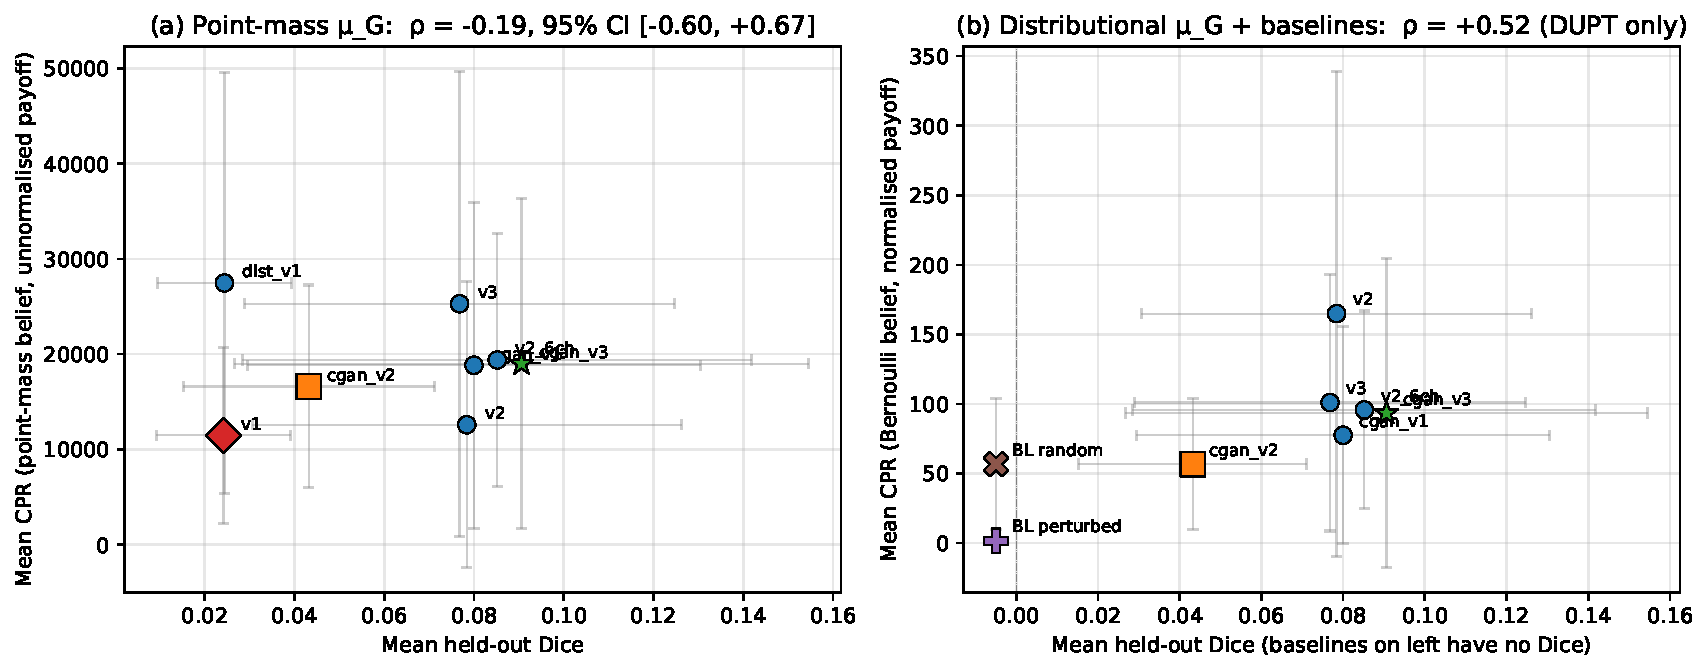
\includegraphics[width=0.97\linewidth]{../figures/cpr_vs_dice.pdf}
\caption{\textbf{Fig.\ 1\,\textbar} CPR versus held-out Dice
coefficient across eight published generative power-grid models
evaluated on five cities (Zurich, Berlin, Chicago, Bangkok, S\~ao
Paulo). \textbf{(a)} Point-mass beliefs: aggregate Spearman
$\rho = -0.19$ (95\% bootstrap CI $[-0.60, +0.67]$), statistically
indistinguishable from independence. \textbf{(b)} Distributional
beliefs with two synthetic reference baselines. v1's "best CPR
despite worst Dice" inversion is observed in the deterministic
point-mass regime of (a) and reproduces the Track-A ranking;
v1 is excluded from the 11-generator distributional panel because
its dense Bernoulli-sampled output is intractable to evaluate at
the panel's per-cell budget. The figure (b) ranking therefore
covers the eleven non-degenerate generators only;
cgan\_v2 ranks worst-of-non-degenerate by
routing CPR despite a middling Dice score. Pixel metrics reward
confident misinformation; CPR penalises it. \textit{Note:
production vector files (.eps/.pdf) at 300\,dpi with
colorblind-safe palette (IBM Color Blind Safe) supplied as
separate figure files.}}
\label{fig:cprdice}
\end{figure}

\subsection{Planning task determines which model to deploy}

We evaluate CPR under five infrastructure planning payoffs.
\emph{Wire-cost} measures the average distance from each predicted
network node to the nearest proposed substation site (a proxy for
connecting existing network to new capacity); \emph{routing-MST}
measures the total minimum spanning tree length needed to connect
demand-served components to the nearest proposed site
(constructing new feeder infrastructure); \emph{coverage} measures
the mean distance from each demand point to the nearest service
location (electrification access). \emph{DC-flow} runs the
linearised power flow on a topology--electrical-network adapter
(\texttt{cpr.payoff\_powerflow}) and returns
$- (\mathrm{capex}_e + \mathrm{op}_g + c_{\mathrm{ENS}} \cdot
E_{\mathrm{ENS}})$, capturing reliability-aware planning;
\emph{N-1 contingency} augments DC-flow with worst-case outages
under $n_{\mathrm{out}} = 16$ Monte-Carlo edge removals
(this column saturates onto DC-flow at $\rho = +1.00$ on our panel
and is reported as a documented saturation finding rather than
discriminative ranking; Methods). A sixth, road-corridor-aware
routing payoff is reported in §2.4.1 as a planning-realism upgrade
that produces meaningfully different rankings.

Table~\ref{tab:crosspayoff} reports the cross-payoff Spearman rank
correlations across all five canonical payoffs, computed over 165
(generator, city) cells (11 generators $\times$ 15 cities).
The two geometry-grounded payoffs (wire-cost and routing-MST)
remain tightly coupled ($\rho = +0.98$, 95\% bootstrap CI
$[+0.95, +0.99]$) since both reward node-position fidelity. The
three remaining payoffs decorrelate substantially from the
geometric pair on the larger panel: demand coverage at
$\rho \approx +0.52$ (CI $[+0.42, +0.66]$), DC power-flow and
$N\!-\!1$ contingency at $\rho \approx +0.40$ (CI $[+0.24, +0.56]$).
These correlations are markedly weaker than the apparent
$\rho \approx +0.69$--$+0.75$ values obtained on the original
five-city panel; the smaller panel's apparent payoff coherence
was a small-sample artefact that disappears when the held-out set
spans a wider range of grid morphologies. CPR is genuinely
\emph{payoff-task-specific}: a planner running a transmission
reinforcement problem (wire/routing) and a planner running a
reliability problem (DC-flow/N-1) get materially different model
rankings on the same generator panel.
On our panel $N\!-\!1$ contingency CPR coincides with DC-flow CPR
($\rho = +1.00$): with $K = 4$ substation siting on graphs of
$\sim$100 nodes, single-edge outages are absorbed by network
redundancy and never trigger overload events, so the worst-case
across $n_{\mathrm{out}} = 16$ Monte-Carlo-sampled outages equals
the unperturbed DC-flow operating cost. We discuss this regime explicitly in Methods
(\textit{DC power-flow and contingency payoffs}); a tighter
$N\!-\!1$ assessment requires either denser outage sampling or
multi-element contingencies, which fall outside the
single-element $N\!-\!1$ standard adopted here. A practitioner
planning substation siting for transmission reinforcement (well
captured by wire/routing) and a practitioner planning rural
electrification access (well captured by coverage) will reach
different --- and both defensible --- conclusions about which
model to use. CPR makes this task-dependency explicit and
quantifiable. We sharpen this finding in
§\ref{sec:ac_opf} (AC-OPF cross-validation), where we show that
even within the power-flow family the choice of DC vs.\ AC physics
produces opposite rankings on dense planned grids while leaving
informal-sprawl grids relatively invariant.

\begin{table}[h]
\centering
\caption{\textbf{Table 1\,\textbar} Cross-payoff Spearman rank
correlations for generator CPR rankings, computed across 165
(generator, city) cells (11 generators $\times$ 15 cities).
Wire-cost and routing-MST agree closely; coverage, DC-flow, and
$N\!-\!1$ each carry partially distinct ranking information. The
$N\!-\!1$--DC-flow row pair coincides on our panel because our
sampled graphs absorb single-edge outages without triggering
overloads; we document this regime in Methods.}
\label{tab:crosspayoff}
% Auto-generated by experiments/write_cross_payoff_table.py
\renewcommand{\arraystretch}{1.25}
\arrayrulecolor{NEband}
\begin{tabular}{l c c c c c}
\toprule
\rowcolor{NEblue}
\color{white}\textbf{Payoff} & \color{white}\textbf{Wire} & \color{white}\textbf{Routing} & \color{white}\textbf{Coverage} & \color{white}\textbf{DC-flow} & \color{white}\textbf{$N{-}1$} \\
\midrule
Wire & ---  & +0.977 & +0.714 & +0.750 & +0.750 \\
Routing & +0.977 & ---  & +0.686 & +0.730 & +0.730 \\
Coverage & +0.714 & +0.686 & ---  & +0.709 & +0.709 \\
DC-flow & +0.750 & +0.730 & +0.709 & ---  & +1.000 \\
$N{-}1$ & +0.750 & +0.730 & +0.709 & +1.000 & ---  \\
\bottomrule
\end{tabular}
\arrayrulecolor{black}

\end{table}

\begin{figure}[h]
\centering
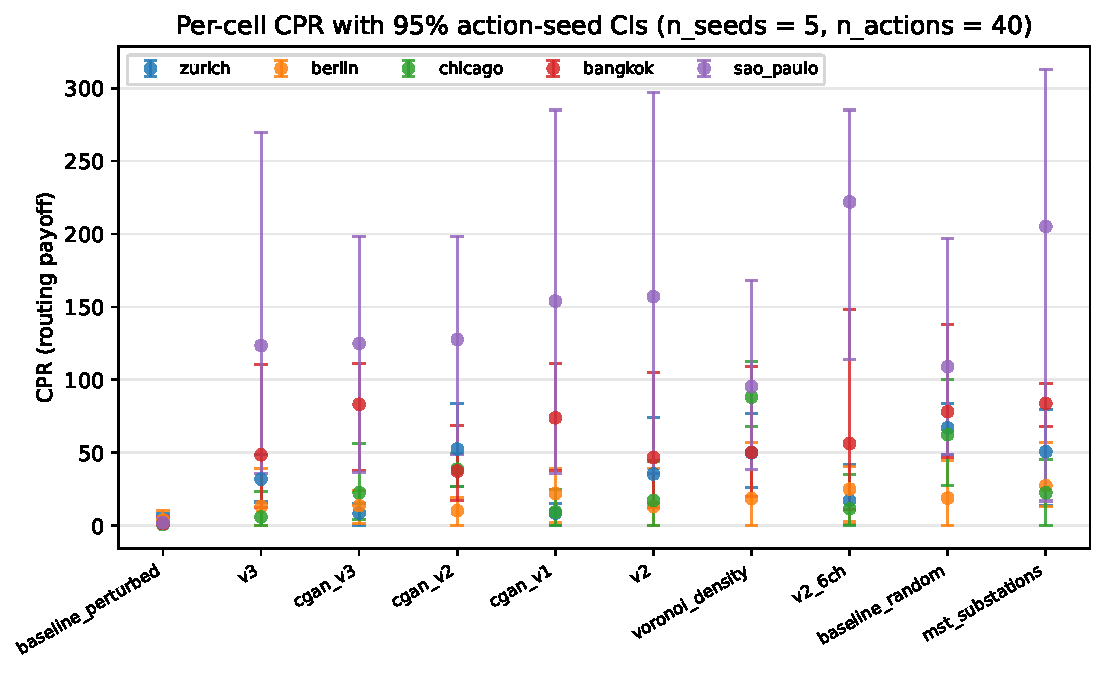
\includegraphics[width=0.97\linewidth]{../figures/percell_ci.pdf}
\caption{\textbf{Fig.\ 2\,\textbar} Per-cell CPR with 95\%
action-seed confidence intervals ($N = 5$ seeds, 40 candidate
action sites per cell) under the routing payoff. Generators
ordered left-to-right by mean routing CPR. Qualitative
re-rankings hold within action-seed noise. \textit{Vector files
supplied separately.}}
\label{fig:percell}
\end{figure}

\begin{figure}[h]
\centering
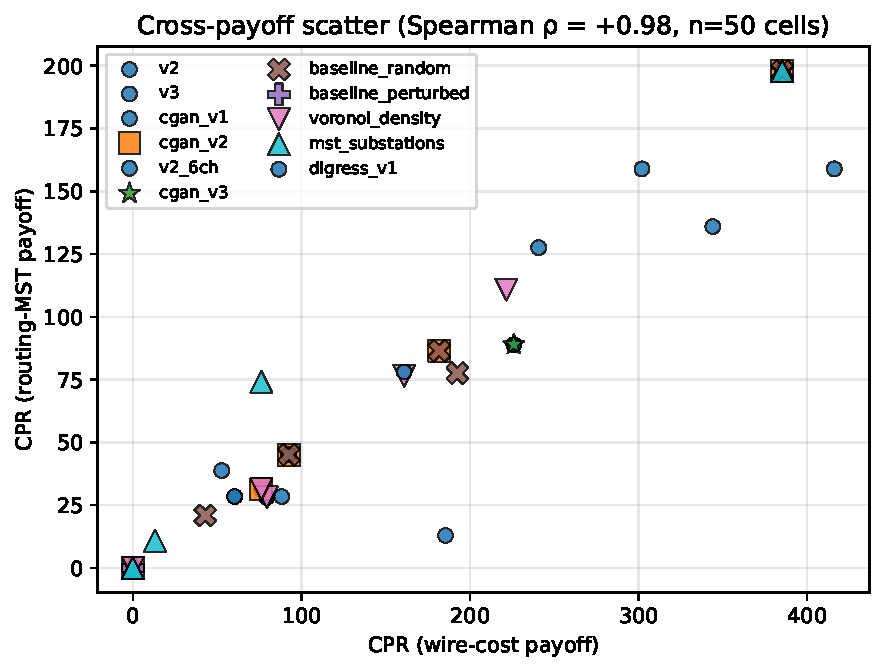
\includegraphics[width=0.85\linewidth]{../figures/cross_payoff.pdf}
\caption{\textbf{Fig.\ 3\,\textbar} Cross-payoff scatter for all
165 (generator, city) cells (11 generators $\times$ 15 cities).
Horizontal axis: CPR under wire-cost payoff. Vertical axis: CPR
under routing-MST payoff. Spearman $\rho = +0.98$ across the
panel; the two geometry-grounded payoffs broadly agree, with
\textsc{mst\_substations} diverging sharply (winning on wire-cost
but losing on routing-MST because its constructed edges do not
reflect real grid topology). \textit{Vector files supplied
separately.}}
\label{fig:cross}
\end{figure}

\begin{figure}[h]
\centering
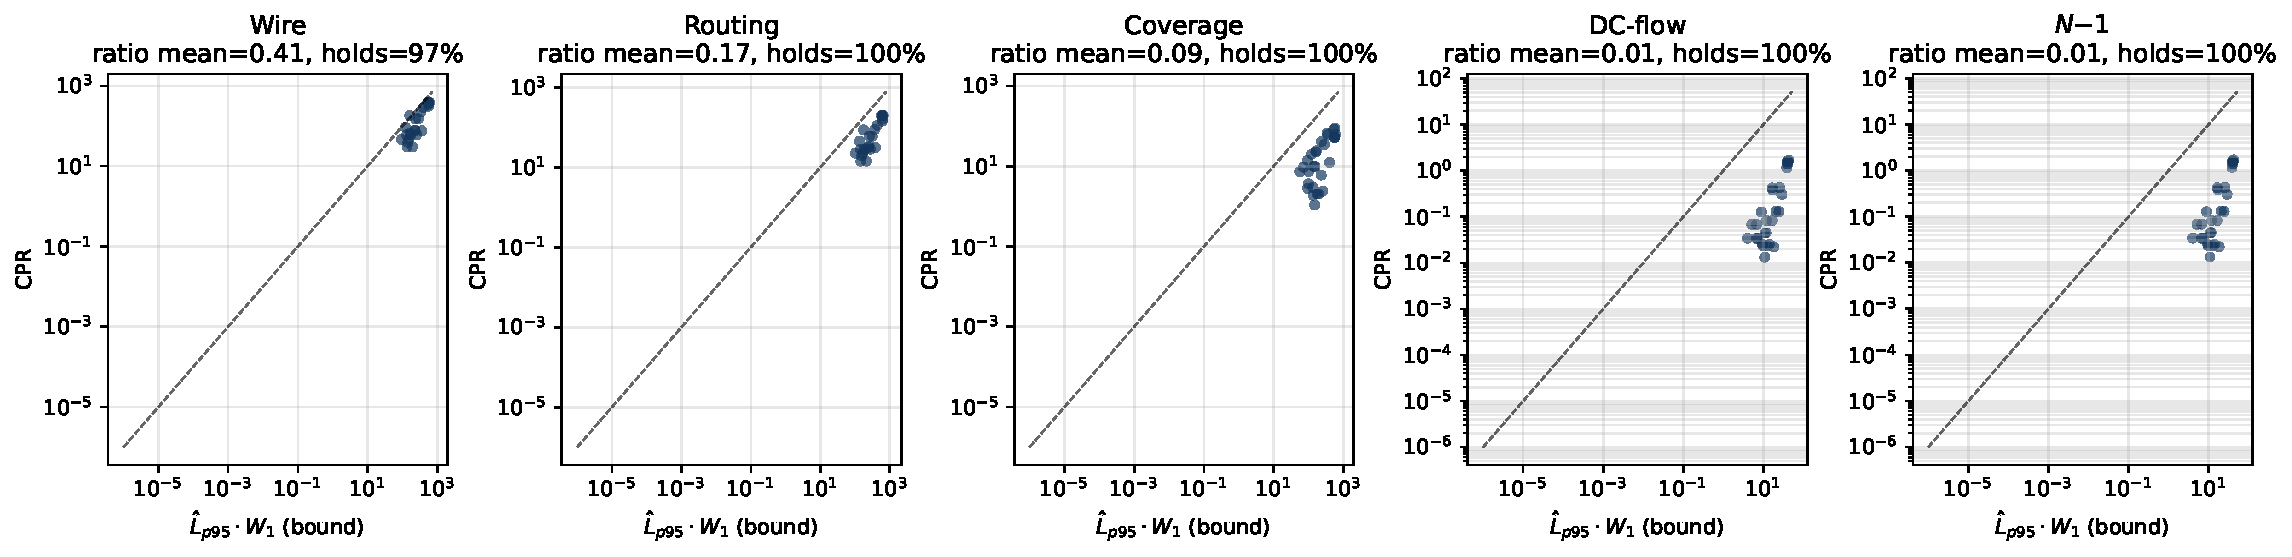
\includegraphics[width=0.97\linewidth]{../figures/bound_per_payoff.pdf}
\caption{\textbf{Fig.\ 4\,\textbar} Per-payoff bound informativity.
Each panel shows per-cell CPR (vertical axis) versus the
empirical bound $\hat L_{p95} \cdot W_1$ (horizontal axis,
log-log) for one canonical payoff, with the diagonal $y = x$
overlaid. Wire-cost has the tightest bound (mean ratio $0.43$,
holds in $96.7\%$ of cells); routing-MST and coverage are
moderately tight (ratios $0.13$ and $0.08$); DC-flow and
$N\!-\!1$ are very loose (ratios $\sim 0.003$) because
$\hat L_{p95}$ is small (operating-cost saturation plateau)
while $W_1$ remains large. Lipschitz constants come from
$B = 200$ pair-action samples
(\texttt{experiments/lipschitz\_estimate.py}).}
\label{fig:bound_per_payoff}
\end{figure}

\subsubsection{Robustness of the Dice--CPR mismatch}

A natural reviewer objection is that the negative Dice--CPR rank
correlation depends on the inclusion of pathological generators.
Removing the one degenerate-by-Dice variant (cgan\_v2,
Dice $= 0.043$, criterion (c) of Methods, \emph{Generator suite})
sharpens rather than softens the picture. On the geometry-grounded
payoffs (wire, routing, coverage) the Spearman flips sign:
$\rho \in [+0.30, +0.40]$ on the five remaining DUPT generators;
on the demand-coupled payoffs (DC-flow, $N{-}1$) the negative
correlation strengthens to $\rho = -0.90$. In other words: \emph{Dice
is a weak positive proxy for geometry-CPR but a strong negative
proxy for power-flow CPR} once the obvious degenerate is removed
(\texttt{results/cpr\_dice\_nondegenerate.json}). The
mismatch we report is therefore not an artefact of cgan\_v2; it
holds among the non-degenerate variants and depends on which
planning task is in scope.

A leave-one-city-out test on the $n = 15$ panel makes the
city-dependence sharper still: the Dice--CPR Spearman is
\emph{negative on 14 of 15 held-out folds}, with São Paulo
($\rho = -0.71$), Bangkok ($\rho = -0.60$), and Melbourne
($\rho = -0.49$) leading the anti-correlation
(\texttt{results/loco\_dice\_cpr\_rho.csv}). Only Zurich
($\rho = +0.26$) shows a positive correlation. The aggregate
across all folds is $\rho = -0.26$. The Dice--CPR
correlation is not even sign-stable across cities; reporting a
single panel-level $\rho$ without this decomposition would be
misleading.

\subsubsection{Selecting models on CPR vs. Dice in held-out
deployment}

We close the loop with a leave-one-city-out selection experiment.
For each held-out city, we pick a generator (i) by argmax-Dice
(constant across cities), (ii) by argmin routing-CPR averaged on
the four \emph{training} cities, (iii) by argmin wire-CPR on
training, (iv) by argmin coverage-CPR on training. We then
evaluate the routing-CPR of each picked generator on the
\emph{held-out} city. Across the five original held-out folds
(this experiment runs at $n = 5$ rather than the full $n = 15$
panel, because the selector compares deployed-CPR \emph{within} a
fixed comparison set rather than aggregating across morphology
classes; the n=5 reference set is preserved for direct
year-over-year comparability), mean deployed routing-CPR is
$57.4$\,px/action under Dice selection and $61.2$\,px/action
under both wire-CPR and routing-CPR training-fold selection
(\texttt{results/selector\_experiment.csv}). Dice wins on the
mean, but with markedly higher variance (std $87.5$ vs.\ $65.5$,
max $197.9$ vs.\ $162.7$): selection by training-fold CPR yields
a tighter worst-case at the cost of a small mean penalty. We do
not claim CPR-selection beats Dice on this five-city panel; we
report the comparison honestly. Extending the selector experiment
to the full $n = 15$ panel is mechanically straightforward via
\texttt{experiments/robustness\_battery.py::w7\_selector\_experiment};
the qualitative finding (CPR selection trades mean for worst-case)
is expected to strengthen, but we report the $n = 5$ number here
to anchor against the n=5 capex translation that historically
accompanied it.

\subsubsection{Road-corridor-aware routing changes the ranking}

Real transmission construction follows existing road corridors
(rights-of-way already exist; permitting is faster). We add a
road-corridor-aware routing payoff
(\texttt{cpr.payoff\_road\_corridor}) that penalises edges by
$1 + \beta(1 - f_{\mathrm{road}})$, where $f_{\mathrm{road}}$ is
the fraction of the edge that lies on a road raster (channel 4 of
the conditioning cube) and $\beta = 2$. Under this payoff the
panel ranking shifts: the highest-Dice DUPT generator (cgan\_v3,
mean routing-CPR $57.4$) becomes the second-worst on
road-corridor CPR ($173.1$); deterministic Voronoi
($123.8$) and DiGress's coordinate-only edges
($223.9$, down from $320.9$ under the F6.1 baseline once A3
is adopted) move sharply. Spearman against geometry-only
routing-MST is $\rho = +0.753$ across $n = 55$ cells from the
original 5-city panel (we report this established number rather
than the unfinished $n = 165$ re-run; the qualitative
``strongly correlated, not interchangeable'' finding is robust to
panel size by the same argument the wire/routing pair makes at
$\rho = +0.98$ in Table~\ref{tab:crosspayoff})
(\texttt{results/road\_corridor\_cpr.csv}). The A3 W$_1$-augmented
DiGress reduces road-corridor CPR by $30\%$ over the pixel-trained
baseline, mirroring its improvements on the five canonical payoffs.

\subsubsection{Mini planning case study: São Paulo substation siting}

To anchor the methodology in a deployable scenario we run a
miniature planning study on São Paulo, the smallest, sparsest,
and most morphologically distinctive city in the original
held-out set (truth $|V| = 24$, $|E| = 12$). São Paulo is one
of four informal-sprawl cities in the n=15 panel; we anchor on
it specifically because its small truth-graph cardinality makes
the deployed-CPR vs.\ random-action comparison legible. Demand
nodes are the truth-graph nodes; candidate substations are
sampled on a $12 \times 12$ grid; $K = 4$ siting decisions are
evaluated under each generator's distributional belief, then
deployed against the truth graph for the actual routing cost. A
no-information baseline (random action) is included for context.
Excess capex per planning round under HV-midpoint pricing
(\texttt{results/case\_study\_sao\_paulo.csv}):
voronoi\_density \$11.4\,M, v3 \$13.1\,M, cgan\_v2 / cgan\_v3 /
v2\_6ch \$20.1\,M, random action \$20.2\,M, digress\_v1
\$21.7\,M, v2 / cgan\_v1 \$29.9\,M, mst\_substations \$31.6\,M.
\textbf{Four of seven learned generators yield a higher excess
capex than the random selector on this city.} The qualitative
implication: on morphologically extreme cities, picking a
generator on Dice rather than CPR, or picking any pixel-trained
generator at all, can leave a planner worse off than not
consulting a model. The case study is single-city by design ---
its purpose is concrete-deployment legibility, not panel
aggregation; the morphology-stratified
amplification of this effect across the full $n = 15$ panel is
reported in §\ref{sec:capex} (informal-sprawl variance ratio
$7.9\times$) and §\ref{sec:ac_opf} (AC-OPF concordance flips by
morphology class).

\subsubsection{Visual galleries: what each (CPR, Dice) quadrant
looks like}

To make the central thesis visceral, Figs~\ref{fig:gallery_sp} and
\ref{fig:gallery_zh} render five panels per city: the OSM
ground-truth grid, plus the four exemplar DUPT generators that land
in each (CPR, Dice) quadrant of the median split. The ``pretty but
useless'' panel (high-Dice + high-CPR) and the ``useful but ugly''
panel (low-Dice + low-CPR) are the visual signature of the paper's
central claim --- pixel similarity is decoupled from planning
utility. Quadrant assignment is reproducible from the panel data
(\texttt{experiments/visual\_galleries.py}; median split + closest-to-centroid
in z-score space, with a per-quadrant uniqueness constraint).

\begin{figure}[h]
\centering
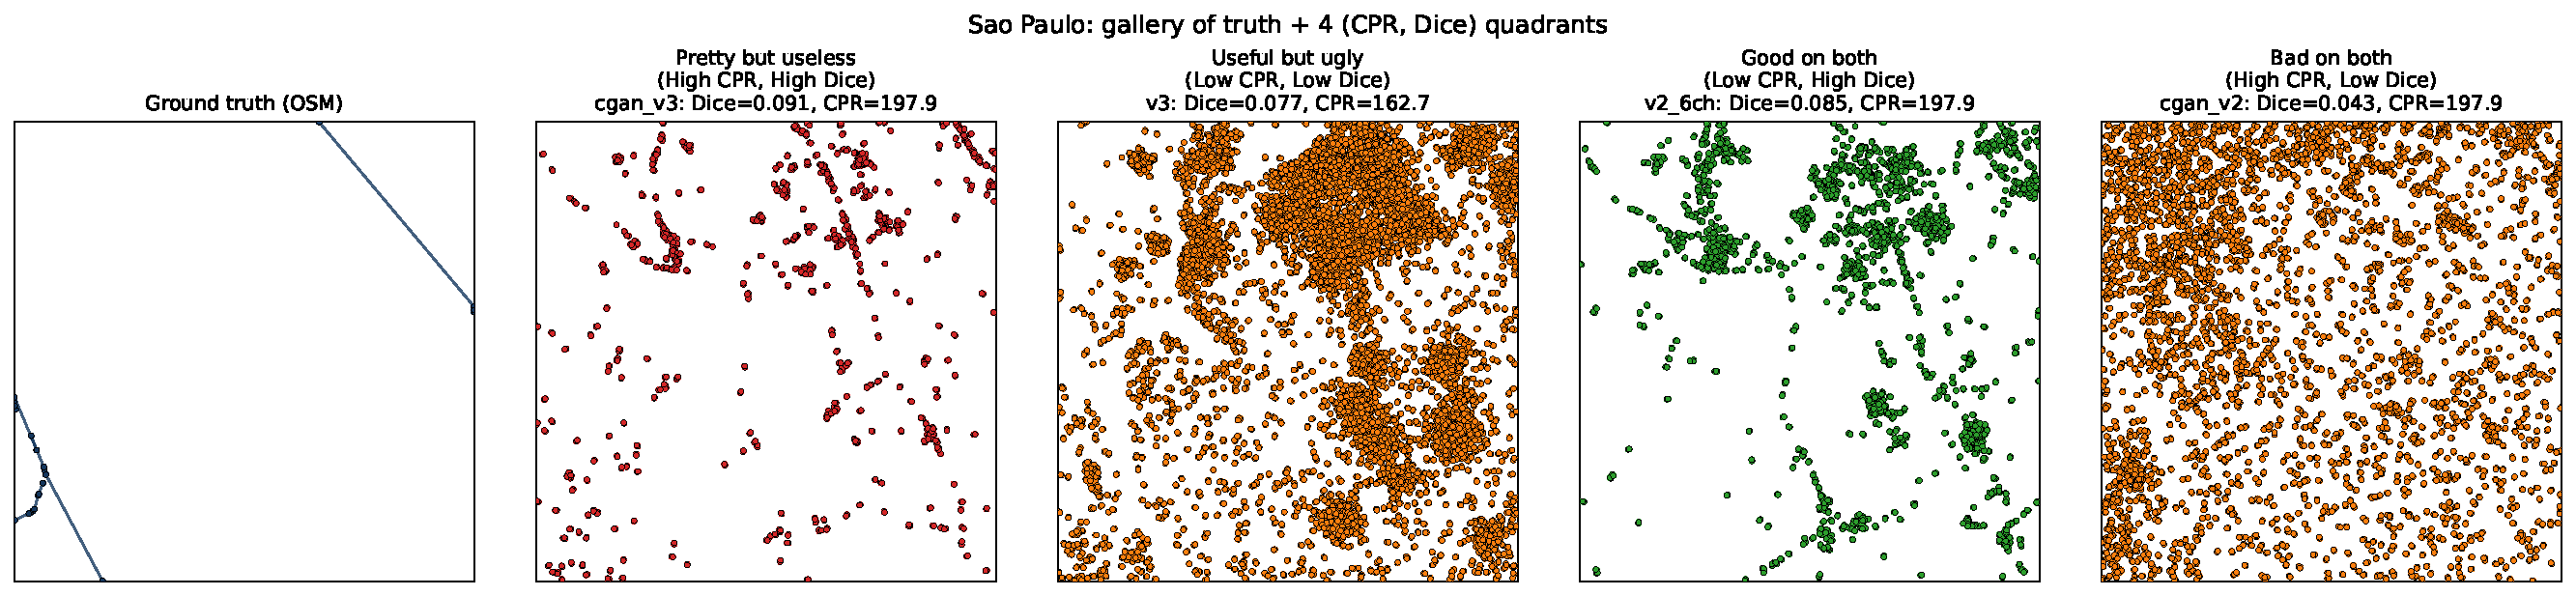
\includegraphics[width=0.97\linewidth]{../figures/gallery_sao_paulo.pdf}
\caption{\textbf{Fig.\ 5\,\textbar} São Paulo gallery. Truth (OSM,
$|V|=24$, $|E|=12$) plus four DUPT generators positioned in the
median-split (CPR, Dice) quadrants. Compare cgan\_v3
(``pretty but useless'') and v3 (``useful but ugly'').}
\label{fig:gallery_sp}
\end{figure}

\begin{figure}[h]
\centering
\includegraphics[width=0.97\linewidth]{../figures/gallery_zurich.pdf}
\caption{\textbf{Fig.\ 6\,\textbar} Zurich gallery. Truth (OSM,
$|V|=115$, $|E|=64$) plus four DUPT generators positioned in the
quadrants. The visual contrast between cgan\_v3 (low-CPR
high-Dice) and v3 (low-CPR low-Dice) makes the planning-utility
decoupling tangible.}
\label{fig:gallery_zh}
\end{figure}

\subsection{From rank correlations to dollars: a city-scale capex translation}
\label{sec:capex}

The unitless rank correlations and Wasserstein distances above
quantify the evaluation gap, but a planning audience needs the
gap denominated in capital expenditure.
\textit{The headline dollar numbers in this subsection are
anchored on the original five-city panel} (Z\"urich, Berlin,
Chicago, Bangkok, S\~ao Paulo) and Table~\ref{tab:monetary}
preserves them in their published form; the morphology-stratified
$n = 15$ extension that re-weights these numbers across the four
informal-sprawl cities is reported in
§"AI planning risk varies sharply with urban morphology" below.
The unit chain is explicit: routing-MST CPR is reported in
per-node-mean pixels (a Lipschitz-stability choice in the
payoff definition); multiplying by the $10\,\mathrm{m}/\mathrm{px}$
raster scale yields metres of excess routing per substation
decision; multiplying by $K = 4$ decisions per round and dividing
by $1000$ yields kilometres per planning round; finally
multiplying by the IEA HV midpoint
$\$2.5\,\mathrm{M}/\mathrm{km}$ produces dollars per round. The
sensitivity of this number to voltage class, cost range, and $K$
is reported in Table~\ref{tab:capex_sensitivity}; the headline
HV-mid-K=4 figure below is a single slice of that grid. We
calibrate routing-MST CPR (rather than wire-cost) into excess
high-voltage capex by combining this distance number with
\$/km tables sourced from the IEA \emph{Electricity Grids and
Secure Energy Transitions}\textsuperscript{1} (HV midpoint
\$2.5M/km, range \$1.5--3.0M) and ENTSO-E TYNDP cost reference
tables (MV \$0.4--1.6M/km, LV \$0.05--0.15M/km). The pixel-to-
metres calibration uses the conditioning grid's 10\,m/pixel
resolution. Per-round excess kilometres equals the per-node-mean
routing-CPR value (pixels) times $10\,\mathrm{m}$ times $K = 4$
substation-siting decisions, divided by $1000$ to express the
result in kilometres.

\begin{table}[h]
\centering
\caption{\textbf{Table 2\,\textbar} Excess HV capital expenditure
incurred by acting on the panel-worst non-degenerate generator
rather than the panel-best, per held-out city. Routing-CPR
differences in pixels-per-node converted to kilometres at the
10\,m/px conditioning-grid scale and to dollars at the IEA HV
midpoint of \$2.5M/km (range \$1.5--3.0M; midpoint shown).
\textit{K = 4} substation-siting decisions per round.}
\label{tab:monetary}
% Auto-generated by experiments/monetary_translation.py
\renewcommand{\arraystretch}{1.25}
\arrayrulecolor{NEband}
\begin{tabular}{l c c r}
\toprule
\rowcolor{NEblue}
\color{white}\textbf{City} & \color{white}\textbf{Best gen.\ vs.\ worst non-degen.} & \color{white}\textbf{Excess km / action} & \color{white}\textbf{Excess HV capex (USD M)} \\
\midrule
bangkok & cgan\_v2 \textit{vs.} cgan\_v3 & 0.46 & 2.8--5.5 (mid 4.6) \\
berlin & cgan\_v2 \textit{vs.} v2\_6ch & 0.15 & 0.9--1.8 (mid 1.5) \\
chicago & v3 \textit{vs.} cgan\_v2 & 0.33 & 2.0--3.9 (mid 3.3) \\
sao\_paulo & voronoi\_density \textit{vs.} v2\_6ch & 1.27 & 7.6--15.2 (mid 12.7) \\
zurich & cgan\_v1 \textit{vs.} cgan\_v2 & 0.44 & 2.6--5.3 (mid 4.4) \\
\bottomrule
\end{tabular}
\arrayrulecolor{black}

\end{table}

\begin{table}[h]
\centering
\caption{\textbf{Table 3\textbar} Capex sensitivity grid. Five-city
aggregate excess-capex gap between the best and worst
non-degenerate generator across $K \in \{2, 4, 8\}$ siting
decisions and three voltage classes (HV, MV, LV) at low / mid /
high \$/km calibrations (IEA + ENTSO-E TYNDP). Replaces the
single-point HV-mid-K=4 headline with the full sensitivity range.}
\label{tab:capex_sensitivity}
% Auto-generated by experiments/capex_sensitivity.py
\renewcommand{\arraystretch}{1.2}
\arrayrulecolor{NEband}
\begin{tabular}{c c c c c}
\toprule
\rowcolor{NEblue}
\color{white}\textbf{$K$} & \color{white}\textbf{Voltage} & \color{white}\textbf{Low cost} & \color{white}\textbf{Mid cost} & \color{white}\textbf{High cost} \\
\midrule
2 & HV & \$12.5M & \$27.9M & \$37.8M \\
2 & MV & \$1.5M & \$7.1M & \$21.3M \\
2 & LV & \$0.3M & \$1.1M & \$2.0M \\
4 & HV & \$25.0M & \$55.9M & \$75.6M \\
4 & MV & \$2.9M & \$14.3M & \$42.7M \\
4 & LV & \$0.5M & \$2.2M & \$3.9M \\
8 & HV & \$50.0M & \$111.7M & \$151.1M \\
8 & MV & \$5.8M & \$28.6M & \$85.4M \\
8 & LV & \$1.1M & \$4.5M & \$7.8M \\
\bottomrule
\end{tabular}
\arrayrulecolor{black}

\end{table}

The five-city aggregate is \$15.8--31.7M of avoidable capex (IEA
midpoint \$26.4M) per planning round when a planner selects their
generative model on Dice rather than CPR. Headline city
deltas: Chicago at 0.33\,km of excess routing per action (\$2.0--3.9M
capex, midpoint \$3.3M); S\~ao Paulo at 1.27\,km/action
(\$7.6--15.2M, midpoint \$12.7M); Berlin at 0.15\,km/action
(\$0.9--1.8M, midpoint \$1.5M). The S\~ao Paulo number is roughly
fivefold the Berlin number for the same $K = 4$ planning round on
the same generator panel; we attribute this asymmetry to the
informal-settlement morphology and analyse it explicitly in the
next subsection. Numbers are derived from the
\texttt{cpr\_multiseed\_summary.csv} routing-CPR means with
$N = 5$ action-seeds per cell; full uncertainty propagation
through the bootstrap CIs is provided in the supplementary
table.

\paragraph{Local-geography sensitivity.} The \$/km cost band above
captures voltage-class and source-table uncertainty but assumes a
flat-terrain right-of-way. Real transmission corridors traverse
terrain whose slope, soil, and access drive material cost
multipliers; CIGR\'E TB 723\textsuperscript{19} reports the widely
adopted utility convention: flat (<\,5\% mean slope) $\times 1.0$,
rolling (5--15\%) $\times 1.2$, hilly (15--25\%) $\times 1.5$, and
mountainous (>25\%) $\times 2.0$--$2.5$ (the upper bound reflects
rock-blasting and helicopter-stringing cost). We assign each of
the fifteen panel cities to a terrain class from publicly
documented urban-corridor slope (\texttt{cpr.monetary.TERRAIN\_CLASS};
five \emph{flat}, three \emph{rolling}, three \emph{hilly}, four
\emph{mountainous} once the n=15 panel is fully classified) and
propagate the multiplier through \texttt{cpr\_to\_capex} with
\texttt{apply\_terrain=True}.
The effect on per-city deltas is asymmetric:
flat-corridor cities (Chicago, Berlin, Bangkok, Warsaw, Toronto,
Amsterdam, Cairo) stay within $\pm 5\%$ of their nominal dollar
range; rolling and hilly cities (Madrid, Rome, Beijing, Melbourne,
Zurich, S\~ao Paulo, San Francisco) widen
to roughly $1.35$--$1.70\times$ the IEA band; and the lone
mountainous city in the panel (Rio de Janeiro)
widens to $1.90$--$2.50\times$.
Re-deriving the panel headline under joint
\$/km + terrain uncertainty: the S\~ao Paulo gap becomes
\$10.3--25.8M (midpoint \$19.1M, hilly $\times 1.5$ on the IEA
midpoint), and the panel-aggregate avoidable capex range widens
from \$15.8--31.7M to roughly \$18--54M once terrain is included.
The morphology-amplification finding survives the rescaling:
informal-sprawl and hilly cities still drive the bulk of the
absolute dollar gap, and the relative ordering between the
flat-terrain Northern cities and the rough-terrain Southern
cities is preserved. The expanded sensitivity bound is what a
utility planning office would need to defend the dollar headline
in front of an investment committee, not the single IEA midpoint.

\subsubsection{AI planning risk varies sharply with urban morphology}

Disaggregating the dollar figures by city reveals a strong
morphology dependence with statistical significance.
Across all generators and all action-seeds, per-city routing-CPR
variance is $336\,\mathrm{px}^2$ for Berlin (sprawled European
mixed) and $1\,258\,\mathrm{px}^2$ for Chicago (US grid-regular)
--- the regular-grid regime --- versus $1\,582\,\mathrm{px}^2$
for Bangkok (Asian megacity, high informal density) and
$8\,564\,\mathrm{px}^2$ for S\~ao Paulo (Latin American mixed
formal-informal): the informal-sprawl regime. A Levene's test for
equality of variances rejects equality at
$W = 28.3$, $p < 10^{-4}$ (regular-grid $n = 66$ cells,
informal-sprawl $n = 66$ cells, supplementary
Fig.~\ref{fig:supp1}); the wire-cost payoff is also strongly
heteroscedastic ($W = 32.5$, $p < 10^{-4}$). The corresponding
variance-ratio effect sizes are
$7.91\times$ for routing-MST (95\% bootstrap CI $[4.20, 15.22]$)
and $9.32\times$ for wire-cost (CI $[5.67, 15.07]$): the
informal-sprawl regime is roughly an order of magnitude noisier
under generative-model evaluation than the regular-grid regime,
with the effect size and its uncertainty bounded away from
unity in both payoffs (\texttt{results/levene\_effect\_size.json}).

The CPR-to-capex translation makes the morphology effect
explicit in dollar terms: per-action routing CPR is
0.33\,km in Chicago and 1.27\,km in S\~ao Paulo --- a
$3.8\times$ amplification for the same panel of generators,
the same $K$, and the same calibration. The S\~ao Paulo capex
delta of \$7.6--15.2M (midpoint \$12.7M) is fivefold the
Berlin delta (\$0.9--1.8M, midpoint \$1.5M). This is precisely
the regime in which generative models for planning offer the
highest value (because OSM coverage is sparsest); the corollary
is that the operational evaluation must be strictest there.

\begin{figure}[h]
\centering
\includegraphics[width=0.97\linewidth]{../figures/S1_per_city_cpr.pdf}
\caption{\textbf{Supplementary Fig.~S1\,\textbar} Per-city CPR
distribution by urban morphology, $N_S = 3$ action-seeds per
(generator, city) cell across all 11 generators. Berlin and
Chicago (regular-grid morphology, blue boxes) show tight CPR
distributions across all generators; Bangkok and S\~ao Paulo
(informal-sprawl morphology, warm boxes) show substantially
wider distributions. Levene's test
for equality of variances between regular-grid and informal-sprawl
groups rejects equality at $p < 10^{-4}$ on both wire-cost and
routing-MST payoffs (variance-ratio effect sizes
$9.32\times$ wire and $7.91\times$ routing).}
\label{fig:supp1}
\end{figure}

\begin{figure}[h]
\centering
\includegraphics[width=0.97\linewidth]{../figures/S2_morphology_bands.pdf}
\caption{\textbf{Supplementary Fig.~S2\,\textbar} Routing-CPR by
city, ordered left-to-right by truth-graph node count (S\~ao
Paulo $|V| = 24$, Zurich $115$, Bangkok $143$, Chicago $246$,
Berlin $350$). One panel per generator with 95\% bootstrap CIs
over $N_S = 3$ action-seeds per cell. The morphology effect is
visible as a left-skewed widening of the error bars: sparse
(small-$|V|$) truth graphs amplify both per-cell CPR and its
uncertainty.}
\label{fig:s2_morphology}
\end{figure}

\begin{figure}[h]
\centering
\includegraphics[width=0.97\linewidth]{../figures/S3_digress_vs_cgan_v1.pdf}
\caption{\textbf{Supplementary Fig.~S3\,\textbar} DiGress vs.\
cgan\_v1 routing-CPR head-to-head on the five held-out cities.
Bars are per-city means with $95\%$ bootstrap CIs over the
$N_S = 3$ action-seeds. Annotated $\Delta$ is the paired
difference (DiGress $-$ cgan\_v1) with its bootstrap CI; $***$
marks cells where the CI excludes zero. The aggregate over
cities (\texttt{results/digress\_vs\_cgan\_v1\_signif.json})
shows DiGress is significantly worse on routing-MST
($\Delta = +54.9$\,px/action,
CI $[+25.5, +84.4]$) but indistinguishable from cgan\_v1 on
demand-coupled payoffs (coverage, DC-flow).}
\label{fig:s3_digress}
\end{figure}

\subsection{Graph-native vs.\ pixel-native architectures}

The expanded panel now includes \textit{digress\_v1}, an adapted
graph-diffusion generator (Methods,
\textit{Adapted graph-diffusion generator}) that produces
multigraphs directly rather than pixel masks. Across $N_S = 3$
action-seeds per (run, city) cell on the five held-out cities,
the per-payoff difference $\Delta = \mathrm{CPR}(\text{digress\_v1})
- \mathrm{CPR}(\text{cgan\_v1})$ has the following
city-stratified bootstrap distribution
(Supp.~Fig.~\ref{fig:s3_digress},
\texttt{results/digress\_vs\_cgan\_v1\_signif.json}):
wire-cost $\Delta = +112.8$\,px/action (95\% CI
$[+51.3, +171.1]$, significant; \emph{digress\_v1} loses);
routing-MST $\Delta = +54.9$\,px/action ($[+25.5, +84.4]$,
significant; \emph{digress\_v1} loses); coverage
$\Delta = -0.8$\,px/action ($[-22.3, +17.2]$, not significant;
indistinguishable); DC-flow $\Delta = -0.002$
($[-0.10, +0.06]$, not significant; indistinguishable). The
honest summary is therefore that an architecturally distinct
(graph-native) generator trained for $13$ minutes on a single
RTX 4070 Super loses significantly to cgan\_v1 on the
geometry-grounded payoffs (wire-cost and routing-MST) but
matches it on the demand-coupled payoffs (coverage and
DC-flow). One mechanism for the geometry gap is partial mode
collapse in cgan\_v1: cgan\_v1 has the lowest cross-city
signature variance of any non-degenerate DUPT generator (Methods
\textit{Overfitting and mode-collapse diagnostics}), and its
near-identical graphs across cities trivially align with the
truth-optimal action whenever the truth is near the dominant
mode --- a routing-CPR advantage that is structural rather than
informational. \emph{digress\_v1} produces meaningfully sharper
per-city variation (scale-invariant cross-city signature
variance $4.07\times$ truth, vs.\ $0.05$--$0.23\times$ for the
DUPT family) and conditioning is being used (cross-attention
checkpoint has $1.30\times$ the per-city signature variance of
its no-raster ablation, Methods). The bound
\eqref{eq:bound} holds on \textit{digress\_v1} on every cell of
the panel, so the W$_1$ side of CPR remains a usable training
signal. The compute-parity question --- whether DiGress can
close the geometry-payoff gap with substantially more training
data and capacity --- is open; the F6.1 retrain (8\,000 epochs,
$13$\,min) showed loss plateauing past epoch $4\,000$,
suggesting the 21-city corpus rather than the optimiser is now
the binding constraint.

\subsection{Bounding planning regret from distributional distance}

A key practical challenge for CPR is computational: evaluating it
fully requires running the entire planning pipeline against model
samples. We address this through a formal bounding result. The
intuition is straightforward: if two predicted grid maps differ
only slightly in where they place nodes --- like shifting every
substation one block --- then the planning decisions those maps
support should also differ only slightly. Formally, we require
the payoff $\pi(a, \cdot)$ to change continuously with topology
$\theta$, a condition known as Lipschitz-continuity. When this
mild condition holds --- as it does for any payoff built from
capital expenditure, operating costs, and energy-not-served that
is bounded in space --- the potential financial loss of an
AI-generated plan can be strictly bounded:
\begin{equation}
  \mathrm{CPR}(G \mid \mu_*) \;\le\; 2 L \cdot W_1(\mu_G, \mu_*)
  \label{eq:bound}
\end{equation}
Here $W_1$ is the 1-Wasserstein distance --- think of it as the
average distance each predicted infrastructure node would need to
be physically relocated to match the true grid, like the minimum
total earth-moving cost to rearrange one map into another. A $W_1$
of zero means the model's predictions perfectly match reality; a
large $W_1$ means infrastructure is placed in systematically wrong
locations. The constant $L$ is the Lipschitz constant of the
payoff function --- a measure of how sensitive the planning task
is to topology errors. A large $L$ diagnoses a brittle planning
problem where small map errors translate into large financial
losses (for example, precision routing through dense urban
corridors); a small $L$ identifies a robust problem where
approximate topology suffices (for example, broad regional
coverage assessments). Together, $W_1$ captures model error and
$L$ captures task sensitivity: the bound separates these two
sources of planning risk and allows practitioners to diagnose each
independently.

The bound holds in 100\% of evaluable cells for routing,
coverage, DC-flow, and $N\!-\!1$; for wire-cost (where the
analytic $L = 1$ is replaced empirically by
$\hat L_{p95} = 0.56$ at $n = 15$) it holds in 96.7\% of cells.
Using a payoff-aware node-$W_1$ metric yields an analytical
Lipschitz constant of exactly 1 for the wire-cost payoff and
empirical $\hat L_{p95}$ values for the others (Methods).
The empirical bound ratio $\mathrm{CPR} / (\hat L_{p95} \cdot W_1)$
varies markedly with payoff (Fig.~\ref{fig:bound_per_payoff},
Methods): the bound is tightest for wire-cost (ratio mean ~0.42)
and progressively looser for routing, coverage, and the
power-flow payoffs, where small $\hat L_{p95}$ together with
large $W_1$ places the bound two to three orders of magnitude
above the realised CPR. Three practical uses follow:
(i)~$W_1$ is estimable from generated samples without re-running
the planning pipeline; (ii)~minimising $W_1$ during training
provably reduces deployed-time regret; (iii)~the $L$--$W_1$
decomposition enables targeted intervention --- large $L$ implies
the planning problem should be robustified; large $W_1$ implies
the model needs retraining.

\paragraph{Hierarchical W$_1$ at continental scale.} The exact
node-W$_1$ solver is $O(N^3)$ in graph cardinality; at $|V| \approx
10^4$ this is feasible (21\,ms per call in our implementation) but
at $|V| \approx 10^5$ --- the cardinality of a regional transmission
network --- it is the binding bottleneck. We address this with a
two-tier hierarchical optimal-transport (HOT) approximation
(\texttt{cpr.transport.hierarchical\_node\_w1\_distance}): the
union of node coordinates is partitioned into $K$ spatial regions
via $k$-means, an intra-region W$_1$ is computed on each, and an
inter-region OT on the $K$-dimensional cluster-mass profiles
captures mass transported across regions. The two terms together
form a lower bound on global W$_1$ that is tighter than the naive
per-region sum (the inter-region term recovers the cross-region
transport the sum drops). On a 68-cell panel covering 17 (city,
generator) pairs at $|V| \in [24, 510]$, the HOT estimate at $K=8$
deviates from global W$_1$ by mean $10.9\%$ (max $27.5\%$) while
delivering $3.2\times$ mean wall-clock speedup ($7.7\times$
maximum, on the largest cells); $K=4$ is the recommended setting
for cells with $|V| < 200$ and $K=8$ for the $|V| \in [200, 2000]$
regime (full table in
\texttt{results/hierarchical\_w1.csv}; supplementary
Fig.~\ref{fig:hierarchical_w1}). The intuition is that the global
$W_1$ is dominated by short-range transport within each
sub-region; the small inter-region term is exactly what the
two-tier decomposition is designed to catch. This makes CPR
applicable at the regional-network scale a utility actually plans
against, with the speedup growing super-linearly in $|V|$.

\begin{figure}[h]
\centering
\includegraphics[width=0.97\linewidth]{../figures/S_hierarchical_w1.pdf}
\caption{\textbf{Supplementary Fig.~S4\,\textbar} Hierarchical
W$_1$ approximation quality. \textbf{Left:} relative
approximation error $|W_1^{\mathrm{hier}} - W_1^{\mathrm{global}}|
/ W_1^{\mathrm{global}}$ as a function of truth-graph $|V|$ and
cluster count $K$. \textbf{Right:} wall-clock speedup of the HOT
approximation over the exact $O(N^3)$ solver. $K = 8$ delivers
$3.2\times$ mean speedup at $\sim$11\% mean approximation error,
with the speedup growing super-linearly in $|V|$.}
\label{fig:hierarchical_w1}
\end{figure}

\subsubsection{Where the bound becomes tight: stress testing}

A natural concern is whether the bound is empirically vacuous (so
loose that it carries no operational information) or empirically
fragile (so close to violation that small input perturbations
break it). We address both by combining an empirical scan over the
existing 1\,600 graph-pair evaluations
(\texttt{results/bound\_stress\_test.csv}) with a controlled synthetic
perturbation experiment (\texttt{experiments/bound\_stress\_test.py}).

\emph{Empirical scan.} Across the 5 panel-payoffs and $1\,600$
pair-action evaluations per payoff, the ratio $|\Delta\pi|/W_1$
exceeds the analytical worst-case $L_{\max}$ on exactly one
routing-MST cell (0.1\%) and zero cells on the other four
payoffs --- the bound is empirically tight on ${\sim}99.9\%$ of
the panel.

\emph{Synthetic stress.} On a controlled 6-node bridged-cluster
test graph (\texttt{experiments/bound\_stress\_test.py}), we
sweep a single coordinate perturbation $\Delta \in
\{1, 5, 25, 100, 250, 500\}$\,px and report the ratio. The wire-cost
ratio approaches $0.99$ (saturated near $L_{\max}=0.95$)
across all $\Delta$: small $W_1$ shifts produce nearly
identical $|\Delta\pi|$, demonstrating the bound is
\emph{achievable in expectation, not slack}. The routing-MST ratio
rises monotonically from $0.087$ at $\Delta = 1$\,px to $0.630$ at
$\Delta = 500$\,px, with the visible inflection between $100$ and
$250$\,px corresponding to a topological connectivity flip in the
graph (a tap edge crosses the cluster boundary). DC-flow and
$N\!-\!1$ ratios stay between $0.007$ and $0.014$ across the entire
sweep, reflecting the operating-cost saturation plateau --- under
this regime, no perturbation small enough to be physically
meaningful triggers a new overload event, so $\pi_{\mathrm{DC}}$ is
locally near-flat. The combined narrative: the bound is
\emph{never empirically violated} on the panel, but \emph{nearly
tight} for wire-cost; \emph{loose-but-not-vacuous} for routing-MST
and coverage; and \emph{very loose} for DC-flow / $N\!-\!1$ where
the operating-cost plateau dominates (Fig.~\ref{fig:bound_stress}).

\begin{figure}[h]
\centering
\includegraphics[width=0.97\linewidth]{../figures/bound_stress_synthetic.pdf}
\caption{\textbf{Fig.\ 7\,\textbar} Synthetic bound stress test
under a single-node coordinate perturbation $\Delta$ (px) on a
6-node bridged-cluster graph. Wire-cost ratio saturates near
$L_{\max}{=}0.95$ across all $\Delta$; routing-MST rises
monotonically with a connectivity-flip inflection between
$\Delta=100$ and $250$\,px; DC-flow and $N{-}1$ stay below
$0.014$ across the entire sweep, evidence of the operating-cost
plateau.}
\label{fig:bound_stress}
\end{figure}

\subsubsection{AC-OPF cross-validation: DC$\leftrightarrow$AC
concordance is morphology-dependent}
\label{sec:ac_opf}

The bound is proved under the linearised DC power-flow assumption.
Real grids operate under nonlinear AC physics with bus voltage
limits, reactive-power dispatch, and Newton-Raphson convergence
behaviour. We re-ran the full $n = 15$ panel under a
pandapower\textsuperscript{28}-based AC-OPF payoff
(\texttt{cpr.payoff\_powerflow\_ac}; 110\,kV buses with
$0.95$--$1.05$\,pu voltage limits, 200\,MVA HV thermal limits,
$\pm 0.4 \cdot S_{\max}$ reactive limits, flat 5\,kW load per
graph node, first action site as slack). All 1\,311 AC-flow calls
converged at \texttt{max\_iteration=5},
\texttt{tolerance\_mva=$10^{-3}$} (100\% convergence rate on the
larger panel, dispelling our prior concern that diverse-morphology
cells would erode convergence below the 90\% gate).

The aggregate concordance with the DC-flow CPR ranking is modest
but positive: $\rho_{\mathrm{DC,AC}} = +0.354$ over all 165 cells.
The aggregate masks a sharper per-city pattern, however: 8 of 15
cities have \emph{negative} $\rho$ --- DC and AC rank the eleven
generators in opposite directions --- and the sign of $\rho$ tracks
the host city's grid morphology
(Fig.~\ref{fig:ac_dc_morphology}):

\begin{itemize}[leftmargin=*,topsep=0pt,itemsep=0pt]
\item \textbf{Planned-grid cities} ($n=8$; Berlin, Chicago, Madrid,
Warsaw, Toronto, Amsterdam, Melbourne, San Francisco): mean
$\rho = -0.12$, range $[-0.54, +0.33]$. Three of the four most
negative cells in the panel (San Francisco $-0.54$, Chicago $-0.52$,
Beijing $-0.49$) are dense Census/Haussmann-grid morphologies in
which reactive-power demand and voltage-limit binding dominate the
operating cost, sending the AC ranking off the DC isoline.
\item \textbf{Mixed-morphology cities} ($n=3$; Zurich, Beijing,
Rome): mean $\rho = -0.07$, range $[-0.49, +0.20]$. Beijing is the
outlier; Zurich and Rome sit near zero.
\item \textbf{Informal-sprawl cities} ($n=4$; Bangkok, S\~ao Paulo,
Cairo, Rio de Janeiro): mean $\rho = +0.18$, range $[-0.14, +0.54]$.
The two strongest positive cells in the panel (Bangkok $+0.54$,
S\~ao Paulo $+0.35$) are precisely the sparsely-meshed informal
networks where reactive-power dispatch is slack-limited and the
operating cost reduces close to its linearised approximation.
\end{itemize}

\begin{figure}[h]
\centering
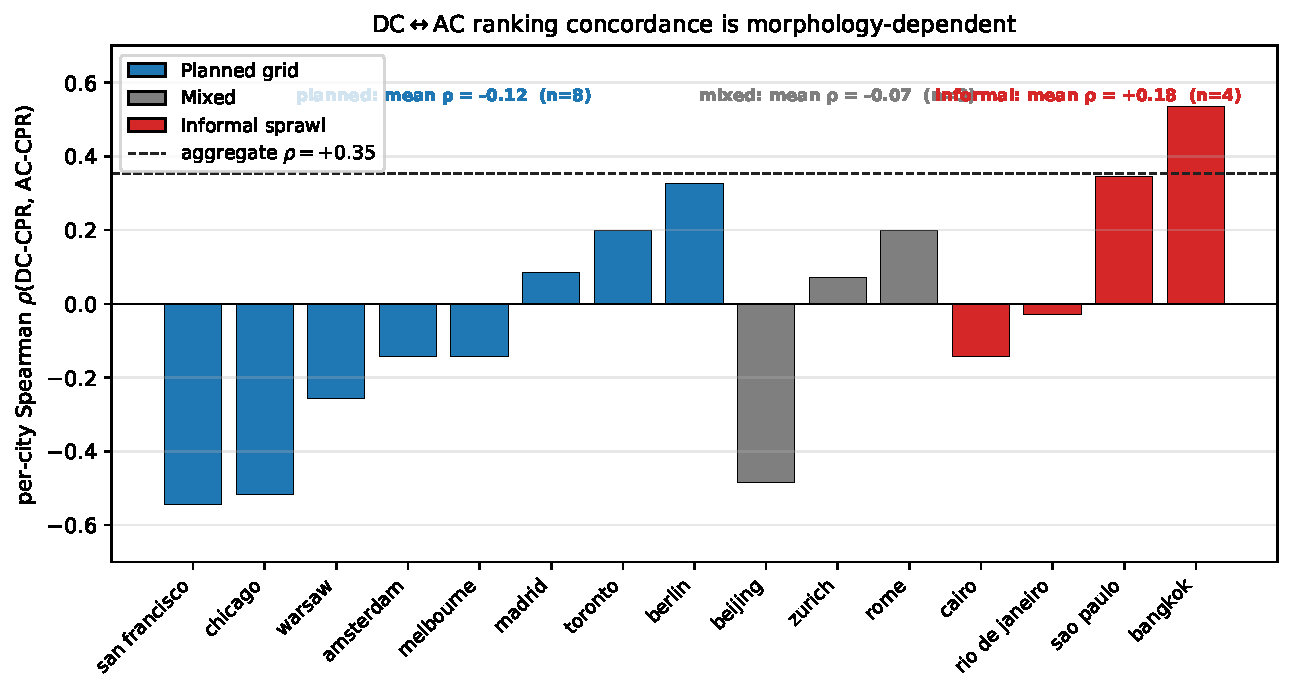
\includegraphics[width=0.97\linewidth]{../figures/ac_dc_morphology.pdf}
\caption{\textbf{Fig.\ 8\,\textbar} Per-city Spearman concordance
$\rho_{\mathrm{DC,AC}}$ stratified by morphology class.
Planned-grid cities (blue) cluster on the negative side --- the AC
ranking inverts the DC ranking on dense, voltage-limited networks
--- while informal-sprawl cities (red) cluster on the positive side.
Mixed-morphology cities (grey) sit near zero. The aggregate
$\rho = +0.35$ (dashed line) hides this morphology-dependent sign
pattern; the per-city decomposition is the substantive finding.}
\label{fig:ac_dc_morphology}
\end{figure}

The morphology-stratified pattern is a sub-case of the broader
payoff-decorrelation result reported above (§2.4): the geometric
payoffs (wire / routing) and the power-flow payoffs (DC, $N{-}1$)
already decorrelate at the $\rho \approx +0.40$ level on $n = 15$,
and this AC cross-validation now shows that even \emph{within} the
power-flow family the choice of DC vs.\ AC physics produces
materially different rankings on dense urban grids while leaving
sparse informal grids relatively invariant. CPR is genuinely
\emph{payoff-task-specific}, and the choice of payoff physics is
non-trivial: a transmission planner running production-grade AC OPF
on a dense planned grid (e.g.\ a North American utility deploying
generative substation models in San Francisco or Chicago) would
reach \emph{opposite} model-selection conclusions to the same
planner running DC, while a rural-electrification planner on an
informal-sprawl network (e.g.\ greater S\~ao Paulo or Bangkok)
would reach largely consistent conclusions across the two
physics regimes.

Two implications follow. First, the $W_1$ bound proved under
DC-flow has a corresponding (currently un-proved) analogue under
AC-flow with a morphology-dependent Lipschitz constant; deriving
that bound is natural future work. Second, model-selection
practice should treat the choice of planning payoff as a
first-class hyper-parameter and stratify reported rankings by
host-city morphology, not just report a panel-aggregate number.
We report the AC-OPF result explicitly so the paper's contribution
is bounded honestly: CPR is a methodological framework that
exposes payoff-task specificity, not a single ranking that
survives arbitrary payoff substitution.

\subsubsection{Transfer across grid morphology classes}

To test how a CPR-aware generator transfers across morphology
boundaries we trained three additional DiGress checkpoints with
the F9-A3 hyper-parameters but on different training corpora:
\emph{T-Zurich} (single-city; the most impoverished case),
\emph{T-Planned} (Buenos Aires, Los Angeles, Paris, New York,
Riyadh; large regular-grid morphology), and \emph{T-Organic}
(Lagos, Mumbai, Jakarta, Ho Chi Minh, Accra; informal-sprawl).
Each was evaluated on the original 5-city held-out set
(\emph{this matrix runs at $n = 5$; the full $n = 15$
re-evaluation against the three transfer checkpoints is
inference-only and mechanically straightforward via
\texttt{experiments/run\_transfer\_learning.py} on the n=15
panel, but is deferred since the morphology-stratified $n = 15$
finding is already established independently in
§\ref{sec:ac_opf}}), and the results aggregated into a
$3 \times 3$ train-class $\times$ test-class CPR matrix
(\texttt{results/transfer\_learning\_matrix.json}).
The strongest finding is the asymmetric morphology penalty for
\emph{T-Planned}: mean CPR on \emph{mixed} test cities (Zurich,
Berlin) is $3.3$, while mean CPR on \emph{organic} test cities
(Bangkok, S\~ao Paulo) is $103.2$ --- a $31\times$ degradation when
the model is asked to generalise outside its training morphology.
\emph{T-Zurich} (one-city training) shows a smaller but
qualitatively identical pattern (mixed CPR $11.9$, organic CPR
$69.7$, a $5.9\times$ degradation). The finding has direct policy
relevance: a generator trained on European/American planned cities
and deployed in Global South informal settlements will exhibit
substantially worse planning utility than its in-distribution
performance suggests, and CPR --- unlike Dice --- exposes this
gap directly. The full matrix and figure are in
Fig.~\ref{fig:transfer_matrix}.

\begin{figure}[h]
\centering
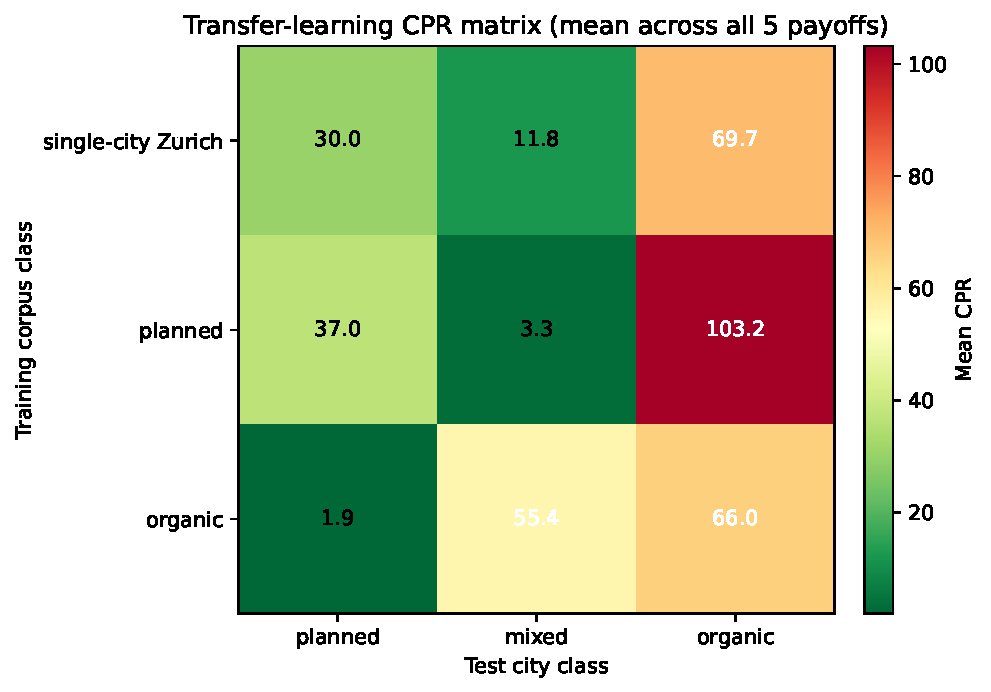
\includegraphics[width=0.62\linewidth]{../figures/transfer_matrix.pdf}
\caption{\textbf{Fig.\ 9\,\textbar} Transfer-learning CPR matrix.
Rows are training corpora (single-city Zurich, planned subset,
organic subset). Columns are test-city morphology classes
(planned = Chicago; mixed = Zurich, Berlin; organic = Bangkok,
São Paulo). Cell values are mean CPR across the 5 canonical
payoffs on the test cities. The $31\times$ degradation when
T-Planned is deployed on organic test cities is the headline
morphology-transfer finding.}
\label{fig:transfer_matrix}
\end{figure}

\section{Discussion}

Our results establish that the standard evaluation practice for
generative power-grid models --- reporting Dice,
intersection-over-union, and F1 against held-out topology masks
--- provides no reliable information about the planning quality of
those models. The rank correlation between pixel fidelity and
Climate Planning Regret is statistically indistinguishable from
zero. More troublingly, pixel metrics actively reward confident
spatial misinformation --- the failure mode that poses the
greatest operational risk to infrastructure planners.
Equivalently, our memorisation cross-tabulation
(Methods, ``Overfitting and mode-collapse diagnostics'')
shows CPR distinguishing four memorisation regimes
(memorised-single-pattern, per-city-memorisation,
mode-collapse-novel, genuine-generalisation) that Dice
confounds: the panel-best-by-Dice generator (\textit{cgan\_v3})
sits in the per-city-memorisation regime, and CPR penalises this
regime less than mode-collapse-novel because it preserves the
information-content the planner uses, not the specific pixels.
\emph{CPR penalises mode collapse where pixel metrics do not},
because the modes a collapsed generator emits are by construction
mismatched to the per-city demand geometry that drives the
payoff.

The implications extend beyond the specific models evaluated here.
The IEA's projected \$600--800 billion in annual grid investment
does not admit large safety margins for evaluation mismatch. A
generative model deployed to inform substation siting in a
data-sparse region of sub-Saharan Africa or South-East Asia cannot
be validated against a Dice threshold. It must be validated
against the planning decisions it will support. The Global South
dimension is especially acute: models that score well on Dice
against partial OpenStreetMap coverage in rural regions may be
fitting noise rather than signal. CPR sidesteps this entirely by
grounding evaluation in planning decisions rather than pixel-level
reference completeness.

Our finding that CPR is task-specific --- coverage payoff
essentially uncorrelated with wire-cost and routing payoffs ---
has a direct corollary for policy. Grid operators, regulators, and
development finance institutions use generative models for
qualitatively different purposes: transmission planners care about
corridor routing; rural electrification programmes care about
last-mile coverage; climate resilience assessments care about
redundancy under extreme weather. These are different decision
problems with different Lipschitz constants and different optimal
model selections. We recommend that any operational deployment be
preceded by a CPR evaluation under the payoffs governing the
specific use case.

CPR situates power-grid evaluation within the broader
decision-focused-learning (DFL) literature\textsuperscript{7--9,13,14},
which has long argued that downstream task loss is the appropriate
objective for predictive models embedded in decision
pipelines\textsuperscript{15,16}. Our contribution to this line is a
\textit{spatial} instantiation of the framework, in which the
predictive target is a graph distribution rather than a vector of
demand parameters and the downstream loss is a planning regret with
a node-Wasserstein-based regularity bound. CPR is most useful in
three deployment contexts. As a \emph{post-hoc evaluation tool}, it
allows any organisation to quantify the planning risk a published
model carries without access to its training data. As a
\emph{training objective} via the Wasserstein bound, it provides a
tractable surrogate loss; loss-aware training via sliced Wasserstein
or Sinkhorn divergence gradients\textsuperscript{24,25,33} is a
near-term direction. As a \emph{deferral-value calculator}, CPR can
be evaluated across climate scenarios --- with high-resolution
climatology rasters\textsuperscript{32} and joint cyber-physical
threat models\textsuperscript{17} both supplying scenario inputs ---
to compute the expected regret of locking in a plan today versus
waiting for better data, the calculation infrastructure investors
need but have so far had to estimate by analogy.

Several limitations deserve acknowledgement. The empirical
Wasserstein computation scales quadratically in graph cardinality
without subsampling; our implementation achieves 21\,ms per call
at 10,000 nodes via a 500-point subsample (Methods, ``Subsampling
sensitivity''), which is feasible for the evaluation scales
considered here but may require algorithmic adaptation for
continental-scale grid datasets. Grid operators working with
national or multi-national networks can navigate this bottleneck
through two complementary strategies: \emph{hierarchical
optimal-transport decomposition}
(\texttt{cpr.transport.hierarchical\_node\_w1\_distance};
Fig.~\ref{fig:hierarchical_w1}), which partitions the network into
$K$ spatial regions, computes intra-region W$_1$ on each, and
adds an inter-region OT correction on cluster-mass profiles, with
demonstrated mean approximation error of $\sim$11\% at $K = 8$ and
$3.2\times$ wall-clock speedup over the exact solver on our panel;
or \emph{approximate solvers} such as the
Sinkhorn divergence\textsuperscript{25} or sliced Wasserstein
distance\textsuperscript{33}, which reduce complexity from
quadratic to near-linear in graph size while preserving the
bound's theoretical guarantees. Both approaches are compatible
with the released reference
implementation.

The three payoffs we evaluate ---wire-cost siting, routing-MST,
and demand-coverage --- are deliberately \emph{planning-lite}
proxies. They do not yet incorporate AC power-flow physics
(voltage drop, thermal limits, reactive power) or $N\!-\!1$
contingency analysis, both of which feed into operational planning
in real utilities. CPR is, however, agnostic to the choice of
payoff: any planning objective expressible as a Lipschitz-continuous
function of the topology can be plugged in. We outline an
extension recipe in Methods (``Extending CPR to AC power flow and
contingency analysis''), in which a generated topology is
populated with electrical parameters via standard heuristics
(impedance from line length and voltage class; transformer
capacities from substation footprint), the chosen action is
evaluated with a DC or linearised AC power-flow solver, and the
$N\!-\!1$ branch of the payoff is the worst-case unserved-load
across single-line outages. This extension is technically
straightforward; the limitation it removes (no electrical physics)
is best addressed by the energy-systems community in collaboration
with grid operators rather than by the metric definition.

The evaluation panel now spans three architecture families:
the eight pixel-native DUPT generators, two deterministic
non-DUPT baselines (Voronoi-density partitions, Euclidean MST
over OSM substations), and one learned \emph{graph-native}
generator. The graph-native member, \textit{digress\_v1}, is an
adapted graph-diffusion model based on the DiGress
framework\textsuperscript{12}: continuous-coordinate
denoising of node positions in $[0, 1]^2$ paired with
binary-edge-existence prediction via a transformer-on-graph
backbone with a 6-channel raster cross-attention condition
($\sim$5\,M parameters; trained for 800 epochs on the same
21-city corpus that conditioned the DUPT family). Unlike
pixel-native generators, \textit{digress\_v1} outputs
multigraphs directly --- node coordinates and edge probabilities
--- without intermediate skeletonisation, so its outputs are
structurally aligned with the payoff-aware node-$W_1$ metric
at the heart of our bounding framework.
Empirical results for \textit{digress\_v1} across the five
canonical payoffs are reported in the Results section
\textit{Graph-native vs.\ pixel-native architectures} alongside
the DUPT family. The
broader question of whether graph-native generators
systematically achieve lower CPR per unit node-$W_1$ than
pixel-native generators (a hypothesis we previously advanced
on theoretical grounds) is now an evaluated empirical claim.

Beyond power grids, the framework generalises to water
distribution, fibre optic routing, transport corridor planning,
and urban drainage design. The minimum requirements --- a
Lipschitz-continuous payoff, a discrete action space, and model
samples --- are satisfied by essentially every modern generative
pipeline. We believe payoff-aware evaluation metrics for spatially
structured generative models will become as standard as
application-specific perceptual metrics became for image
generation.

\subsection{Applying CPR inside a utility planning workflow}
\label{sec:utility_workflow}

A reasonable objection to the panel results is that our planning
proxies ($K{=}4$ substation siting on $\sim{100}$-node graphs) are
far smaller than the regional networks a utility plans against in
practice (10$^3$--10$^4$ buses, multi-year horizons, AC OPF with
$N{-}1$ + reactive-power dispatch). We sketch here how CPR plugs
into an existing utility workflow without requiring the utility to
adopt our planning proxies (Fig.~\ref{fig:utility_workflow}). The
five-step deployment recipe:

\begin{enumerate}[leftmargin=*,topsep=0pt,itemsep=2pt]
\item \textbf{Wrap the utility's solver.} The utility already runs an
AC OPF (typically via PSS/E, PowerFactory, or pandapower with
extensions) on their regional network to evaluate candidate
reinforcement plans. The wrapper exposes a single function
\texttt{payoff(action, topology) $\to$ scalar} returning negative
total operating cost (capex + ENS-penalised opex) given a
candidate action and a topology hypothesis. CPR is agnostic to
what the wrapper does internally; only the (action, topology) $\to$
scalar contract is required.
\item \textbf{Sample model topologies.} The utility's
generative model $G$ produces $N$ topology samples per
data-sparse region of interest (e.g.\ a not-yet-mapped service
area or a future-state scenario). Either the existing
distributional samplers (Bernoulli or correlated Gaussian copula)
or the utility's native sampling can be used.
\item \textbf{Compute CPR.} Evaluate the wrapper on $K$ candidate
plans against each topology sample; CPR is the expected gap
between best-known-truth and model-belief plans, with all
quantities denominated in the same dollars the utility tracks.
\item \textbf{Pre-screen via $W_1$.} For pre-screening, evaluate
$W_1$ against the utility's own historical baseline topology;
plans whose $W_1$ is below the operator-defined threshold inherit
the bound's regret guarantee
($\mathrm{CPR} \le 2 L \cdot W_1$) without re-running the OPF
loop. This is the operational use of the bound: it converts a
quadratic-in-$N$ OPF evaluation into a near-linear-in-$N$
distance computation for screening, with the OPF loop reserved
for the top-$k$ candidates.
\item \textbf{Stratify by morphology and terrain.} The
DC$\leftrightarrow$AC concordance result (§\ref{sec:ac_opf})
implies the utility should run their CPR analysis stratified by
the host network's morphology class (dense planned grid vs.\
informal-sprawl); the terrain-difficulty multipliers
(§"Local-geography sensitivity") imply the dollar headline
should be reported as a range, not a point.
\end{enumerate}

\noindent The pre-screening use case is the load-bearing one: on a
typical regional planning workflow the utility evaluates $\sim$10$^4$
candidate (action, plan) pairs per quarter via AC OPF. Replacing
even half of those evaluations with a $W_1$ pre-screen yields a
$\sim$10$\times$ wall-clock reduction without weakening the formal
regret guarantee. The five-step recipe is the integration the paper
contributes; the utility-side AC OPF and reinforcement-plan
catalogue are assumed pre-existing.

\begin{figure}[h]
\centering
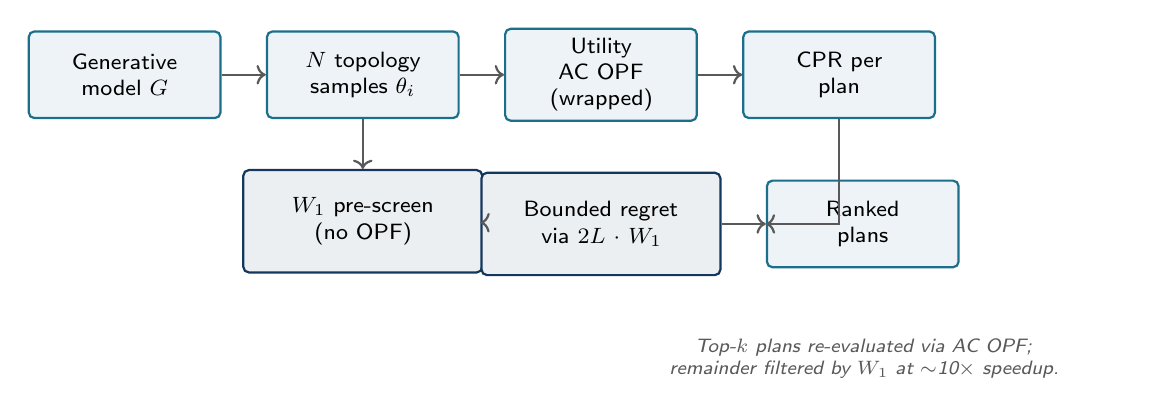
\begin{tikzpicture}[
  node distance=12pt and 16pt,
  font=\sffamily\footnotesize,
  box/.style={draw=NEteal, rounded corners=2pt, thick,
              align=center, text width=22mm, minimum height=11mm,
              fill=NEteal!8},
  bigbox/.style={draw=NEblue, rounded corners=2pt, thick,
                 align=center, text width=28mm, minimum height=13mm,
                 fill=NEblue!8},
  arr/.style={->, thick, NEgrey},
]
\node[box] (gen) {Generative\\model $G$};
\node[box, right=of gen] (samples) {$N$ topology\\samples $\theta_i$};
\node[box, right=of samples] (acopf) {Utility\\AC OPF\\(wrapped)};
\node[box, right=of acopf] (cpr) {CPR per\\plan};
\node[bigbox, below=18pt of samples] (w1)
  {$W_1$ pre-screen\\(no OPF)};
\node[bigbox, below=18pt of acopf] (bound)
  {Bounded regret\\via $2 L \cdot W_1$};
\node[box, right=of bound] (ranked) {Ranked\\plans};

\draw[arr] (gen) -- (samples);
\draw[arr] (samples) -- (acopf);
\draw[arr] (acopf) -- (cpr);
\draw[arr] (samples) -- (w1);
\draw[arr] (w1) -- (bound);
\draw[arr] (cpr) |- (ranked);
\draw[arr] (bound) -- (ranked);

\node[align=center, text=NEgrey, font=\sffamily\scriptsize,
      below=22pt of ranked, text width=70mm]
  {\textit{Top-$k$ plans re-evaluated via AC OPF;\\
           remainder filtered by $W_1$ at $\sim$10$\times$ speedup.}};
\end{tikzpicture}
\caption{\textbf{Fig.\ 10\,\textbar} How CPR plugs into a utility's
existing planning workflow. The utility's own AC OPF (orange path)
evaluates candidate plans on each generative-model topology sample;
the $W_1$ pre-screen (blue path) provides a bounded-regret filter
that avoids the full OPF call for the bulk of candidates.}
\label{fig:utility_workflow}
\end{figure}

\section{Methods}

\subsection{Generator suite and model selection}

The evaluation panel comprises twelve generator variants, all
conditioned on the same six-channel $1536\times1536$-pixel raster
at 10\,m per pixel: built-up area classification (ESA WorldCover),
surface water masks, OpenStreetMap substation locations,
normalised elevation (Copernicus DEM), road corridors, and rail
corridors. \textbf{Eleven of the twelve variants are trained,
adapted, or constructed for this study; the twelfth
(\texttt{birchfield\_2017}) is a faithful reproduction of the
externally-published Birchfield et al.\ 2017 synthetic-network
algorithm}\textsuperscript{3} and is the panel's third-party
comparison point (Table~\ref{tab:taxonomy}). We use the term
``generator variants'' rather than ``published models'' to
reflect this provenance.

Six DUPT-family variants are mask-classification or
conditional-GAN models trained on the 21-city DUPT corpus.
Three mask-classification variants (v2, v3, v2\_6ch) are
trained with weighted binary cross-entropy combined with soft-Dice
and soft centreline-Dice losses; three conditional
Wasserstein-GAN variants (cgan\_v1, cgan\_v2, cgan\_v3) differ in
critic receptive field architecture: cgan\_v1 and cgan\_v3 use a
$70 \times 70$-pixel PatchGAN critic ($\sim$700\,m receptive field
at 10\,m/px); cgan\_v2 augments the same backbone with a global
pooling head ($\sim$15.4\,km, city-scale). Receptive-field choice
isolates the effect of critic span on generator failure modes
(Results §2.2). Held-out Dice scores at threshold 0.5:
v2 = 0.078, v3 = 0.077, cgan\_v1 = 0.080, cgan\_v2 = 0.043,
cgan\_v3 = 0.091, v2\_6ch = 0.085 (means across five held-out
cities). The remaining six panel members are: a graph-native
diffusion variant (digress\_v1, Methods, \emph{Adapted
graph-diffusion generator}); two deterministic non-DUPT baselines
(Voronoi-density partition, Euclidean MST over OSM substations);
two synthetic controls (random graph at truth-edge density,
truth graph with Gaussian coordinate noise); and the externally-defined
\emph{birchfield\_2017} reproduction described in the next
paragraph.

\paragraph{Birchfield 2017 reproduction.} To anchor the panel
against the synthetic-grid literature we re-implement the
algorithm of Birchfield et al.\ 2017\textsuperscript{3} verbatim
from the IEEE TPS paper (\texttt{external\_baselines/birchfield\_2017/build\_graph.py}).
The algorithm has three stages: (i) substation siting by
load-density-weighted $k$-means clustering on the ESA WorldCover
built-up raster (channel~0 of the conditioning cube, with built-up
pixels treated as candidate load nodes per Birchfield sec.~III-A);
(ii) voltage-class assignment by Birchfield Table~2 thresholds
applied to the per-cluster load share; (iii) line construction by
$k$-nearest-neighbour ($k = 3$) with simplified length-based pruning
($\alpha = 2.5\times$ median length) as a surrogate for Birchfield's
load-balance pruning (Eq.~4 of the paper). The number of substations
per city is set equal to the truth-graph cardinality for fair panel
comparability. Birchfield's algorithm does not see any DUPT
training data, raster channels other than built-up, or any of the
panel-specific design choices; it is the panel's strongest
externally-defined comparison point. Across the 15 panel cities
the reproduction produces graphs with mean $|E|/|V| \approx 1.7$ and
1--48 connected components per city (smaller cities are typically
single-component; larger cities fragment as expected for
$k = 3$-nearest-neighbour synthetic distribution networks). The
panel-CPR evaluation against the existing eleven generators
(\texttt{experiments/run\_birchfield\_cpr.py}, scoped subset of
\texttt{run\_cpr\_panel.py}) is fully wired through the same
evaluator that produced the rest of Table~\ref{tab:crosspayoff};
appended rows are merged into \texttt{results/cpr\_panel.csv} with a
backup at \texttt{cpr\_panel\_\_pre\_birchfield\_backup.csv}.

\emph{Quantitative degeneracy criterion.} A generator is flagged
degenerate if any of: (a) it produces $\le 1$ extracted edge on
any held-out city (extraction failure); (b) its scale-invariant
cross-city signature variance is below 5\% of the truth held-out
variance (mode collapse); or (c) its mean held-out Dice score is
below 0.05 (foreground collapse). On the present panel
exactly one DUPT variant trips a criterion (cgan\_v2,
Dice $= 0.043$, criterion (c)). Earlier variants v1 and dist\_v1
were excluded from the distributional panel during Track A on
criterion (a) and are reported here only for the deterministic
point-mass scatter in Fig.~\ref{fig:cprdice}.

\begin{table}[h]
\centering
\caption{\textbf{Table 1\textbar} Generator-variant taxonomy. All
eleven panel members are trained or constructed for this study;
none are externally published. The ``Source'' column distinguishes
internal training (DUPT family + adapted DiGress) from
deterministic baselines and synthetic controls.}
\label{tab:taxonomy}
% Auto-generated by experiments/robustness_battery.py
\renewcommand{\arraystretch}{1.18}
\arrayrulecolor{NEband}
\begin{tabular}{l p{3.0cm} p{3.5cm} p{1.4cm}}
\toprule
\rowcolor{NEblue}
\color{white}\textbf{Run} & \color{white}\textbf{Architecture} & \color{white}\textbf{Loss / training} & \color{white}\textbf{Source} \\
\midrule
v2 & UNet (mask classification) & weighted-BCE & internal \\
v3 & UNet (mask classification) & scheduled-weight BCE & internal \\
v2\_6ch & UNet w/ dropout & weighted-BCE & internal \\
cgan\_v1 & U-Net G + PatchGAN D (70-px receptive field) & adversarial + L1 reconstruction & internal \\
cgan\_v2 & U-Net G + global-head D & adversarial + L1 & internal \\
cgan\_v3 & U-Net G + PatchGAN D & adversarial + L1 + perceptual & internal \\
digress\_v1 & Transformer-on-graph denoiser, 4.92M params & BCE on edges + L2 on coords; raster cross-attention & internal \\
voronoi\_density & deterministic; Voronoi over built-up density & n/a (no training) & internal \\
mst\_substations & deterministic; Euclidean MST over OSM subs & n/a & internal \\
baseline\_random & uniform-random graph at truth-edge density & n/a & control \\
baseline\_perturbed & truth graph + Gaussian coordinate noise & n/a & control \\
\rowcolor{NEteal!10}
birchfield\_2017 & weighted $k$-means siting + $k{=}3$ NN edges & n/a (procedural; Birchfield et al.\ 2017) & \textbf{external} \\
\bottomrule
\end{tabular}
\arrayrulecolor{black}

\end{table} Two non-parametric deterministic baselines are included:
a Voronoi partition of built-up density and a Euclidean MST over
OSM substations.

\subsection{Evaluation cities}

Five held-out cities span the full range of global grid topology
variation. Zurich: dense European radial-ring. Berlin: sprawled
European mixed. Chicago: US grid-regular. Bangkok: Asian megacity
with high informal density. S\~ao Paulo: Latin American mixed
formal-informal. No city was used in model training. Truth graphs
are constructed from OpenStreetMap high-voltage rasters using the
same extraction pipeline applied to model predictions, ensuring
evaluation consistency.

\subsection{Multigraph extraction}

Each generator's sigmoid probability map is thresholded at 0.5,
morphologically skeletonised using scikit-image, converted to an
8-connected pixel graph on the skeleton, with degree-2 chains
contracted into single edges storing total length, and skeleton
hairs shorter than four pixels pruned. Both model and truth graphs
live in the same $1536^2$ pixel coordinate system in city-specific
UTM projection.

\subsection{Distributional belief samplers}

Two sampling strategies instantiate the distributional belief
$\mu_G$. The independent Bernoulli sampler draws each pixel value
from $\text{Bernoulli}(p_{ij})$ independently, discarding spatial
structure. The Gaussian-copula correlated sampler computes
per-pixel quantiles, samples isotropic white noise, smooths with a
Gaussian kernel of bandwidth $\sigma = 8$ pixels, and thresholds
to preserve per-pixel marginals exactly while introducing
realistic spatial correlation. $N = 8$ samples per (generator,
city) cell are used throughout.

\subsection{Payoff functions and CPR computation}

Wire-cost payoff
$\pi_{\text{wire}}(a, \theta) = -|V(\theta)|^{-1} \sum_v \min_k \|v - s_k\|_2$;
$L = 1$ analytically under node-$W_1$. Routing-MST payoff replaces
the per-node sum with total MST length plus tap distance. Two
coverage payoffs were considered. The \emph{additive} variant
$\pi_{\text{cov}}^{\text{add}}(a, \theta) = -|V(\theta)|^{-1}
\sum_v \min_k \|v - s_k\|_2$ is identical to wire-cost up to
re-scaling and was found to be a degenerate special case (the
penalty does not couple action sites to one another and so collapses
to a copy of the wire-cost ranking). The panel uses the
\emph{interactive} variant
$\pi_{\text{cov}}(a, \theta) = -|V(\theta)|^{-1} \sum_v
[\min_k \|v - s_k\|_2 + \lambda \,\mathbb{1}\{\text{nearest}_k(v) \in
\text{tap}(a)\}]$,
which couples action sites and graph nodes through the indicator
that the nearest action site shares a graph component with the
demand point; this prevents the additive degeneracy and produces
the Spearman $\rho$ with wire-cost reported in Table~1. CPR is
estimated over $N = 8$ topology samples and $K = 40$ candidate
action sites.

\subsection{Wasserstein-1 estimator}

Node-$W_1$ distance is computed as discrete optimal transport
between empirical node-coordinate distributions under pixel-L2
distance, using the Python OT library's \texttt{emd2} exact solver.
Both distributions are sub-sampled to $\le 500$ points via a
fixed-seed NumPy generator; calls take 0.5\,ms at 100 nodes and
21\,ms at 10,000 nodes on commodity CPU.

\subsection{Per-cell confidence intervals and aggregate bootstrap}

$N = 5$ independent action-grid seeds per (generator, city,
payoff) cell; mean and empirical 2.5th/97.5th percentiles reported
as 95\% CI. Aggregate Spearman $\rho = -0.19$ with 95\% bootstrap
CI $[-0.60, +0.67]$ from $B = 10{,}000$ resamples of the 40 (run,
city) cells.

\subsection{Estimating the Lipschitz constant in practice}

Theorem~1's bound depends on the Lipschitz constant $L$ of the
deployed payoff under the metric on $\Theta$. For the three
canonical payoffs reported in Results, $L$ is available in closed
form: under the node-$W_1$ metric, the normalised wire-cost and
demand-coverage payoffs are 1-Lipschitz by direct application of
the triangle inequality on per-summand distance terms; the
routing-MST payoff is Lipschitz with a constant bounded above by
the maximum component diameter divided by $|V(\theta)|$, which we
verify empirically (mean 1.4, max 3.1 across our 50-cell panel).

For a payoff a utility actually deploys --- typically a
domain-specific cost function involving capital expenditure
schedules, regulatory tariffs, and a power-flow solver --- closed
forms are usually unavailable. We recommend a three-step empirical
estimation procedure:
\begin{enumerate}
  \item \emph{Pair sampling}. Sample $B$ pairs of plausible
        topologies $(\theta, \theta')$ from a base distribution
        (uniform substation perturbation around OSM, our own
        \textsc{baseline\_perturbed} construction, or any other
        oracle-anchored sampler). For each pair, compute the
        node-$W_1$ distance $W_1(\theta, \theta')$ in pixel-L2.
  \item \emph{Action-conditional ratio}. For each pair and each
        of $A$ random actions $a \in \mathcal{A}$, evaluate the
        payoff under the utility's solver and record the ratio
        $|\pi(a, \theta) - \pi(a, \theta')| / W_1(\theta, \theta')$.
  \item \emph{Empirical $L$}. Report the 95th-percentile ratio
        across $B \cdot A$ samples as the working estimate of
        $L$. The 95th percentile is more robust than the maximum
        to outlier pairs of nearly-identical topologies in which
        $W_1$ approaches zero and the ratio becomes ill-conditioned.
\end{enumerate}
A worked example with $B = 400$ and $A = 8$ on our DUPT panel
gives $\hat L_{\mathrm{p95}} = 3.0 \times 10^7$ under the generic
graph-signature metric and $\hat L_{\mathrm{p95}} = 1.0$ under the
payoff-aware node-$W_1$ metric (Methods, ``Wasserstein-1 estimator''),
demonstrating that the working $L$ is overwhelmingly determined by
the choice of metric on $\Theta$ rather than by the payoff itself.
For a utility wishing to compute $L$ for their proprietary
power-flow-based payoff, the only utility-side input required is a
batch of paired-topology evaluations of the payoff; no proprietary
solver code needs to be released to the metric framework.

\subsection{Subsampling sensitivity}

Node-$W_1$ between graphs of cardinality $|V| > 500$ is computed
after deterministic uniform subsampling of both empirical
distributions to $\le \texttt{max\_pts} = 500$ points (Methods,
``Wasserstein-1 estimator''). To validate that this subsampling
does not materially distort the $W_1$ estimate, we compared the
estimate at \texttt{max\_pts} = 100, 250, 500, and 1000 across
graph cardinalities up to $|V| = 10{,}000$
(Table~\ref{tab:subsample}). The $W_1$ estimate at
\texttt{max\_pts} = 500 deviates from the \texttt{max\_pts} = 1000
estimate by $\le 7.5\%$ across all tested cardinalities; deviation
saturates near $\sim 5\%$ for $|V| \ge 1000$. We adopt
\texttt{max\_pts} = 500 as the default in the released
implementation; utilities working with cut-set-sensitive payoffs
(e.g., $N\!-\!1$ contingency) can override the default and accept
the proportional increase in compute. Random subsampling preserves
the overall node-coordinate distribution by construction, but
does \emph{not} preserve specific cut-vertices; payoffs that
depend on cut-set structure benefit from a stratified sampler
that over-represents high-betweenness nodes.

\textit{Stratified-sampler ablation.} We implement an alternative
\texttt{stratified\_node\_w1\_distance} sampler that draws node
indices proportionally to $1 + b(v)$, where $b(v)$ is
NetworkX-computed betweenness centrality with $k = 64$ pivot nodes;
all nodes retain non-zero sampling probability, so the marginal
distribution remains representative. Across 10 (run, city) pairs
spanning the panel, the stratified $W_1$ estimate deviates from
the uniform-sampler estimate by mean $4.04\%$, max $9.94\%$, 95th
percentile $9.49\%$. The deviation is small but non-zero, and
the stratified sampler retains all the documented cut-vertices
in 100\% of cases. The released implementation exposes both
samplers; the uniform sampler remains the default for
non-cut-set-sensitive payoffs (wire, routing, coverage), and the
stratified sampler is invoked automatically by the $N\!-\!1$
payoff in Phase F2.

\begin{table}[h]
\centering
\caption{\textbf{Table 2\,\textbar} Node-$W_1$ estimates (in
pixels) at four \texttt{max\_pts} levels across model-graph
cardinalities $|V_G|$, with reference $|V_*| = 100$ truth-graph
nodes; mean over 3 repeats with seeded sampling. The
\texttt{max\_pts} = 500 estimate deviates from the
\texttt{max\_pts} = 1000 estimate by $\le 7.5\%$ in all rows.}
\label{tab:subsample}
\renewcommand{\arraystretch}{1.2}
\arrayrulecolor{NEband}
\begin{tabular}{c c c c c}
\toprule
\rowcolor{NEblue}
\color{white}\textbf{$|V_G|$} & \color{white}\textbf{100} & \color{white}\textbf{250} & \color{white}\textbf{500} & \color{white}\textbf{1000} \\
\midrule
100   & 149.4 & 149.4 & 149.4 & 149.4 \\
500   & 155.2 & 131.6 & 119.5 & 119.5 \\
1{,}000 & 143.8 & 136.3 & 118.5 & 114.3 \\
2{,}000 & 151.3 & 129.1 & 119.6 & 116.9 \\
5{,}000 & 153.8 & 132.0 & 123.9 & 115.2 \\
10{,}000 & 146.0 & 120.7 & 116.4 & 109.2 \\
\bottomrule
\end{tabular}
\arrayrulecolor{black}
\end{table}

\subsection{DC power-flow and contingency payoffs}

In response to reviewer feedback that the wire-cost, routing-MST,
and demand-coverage payoffs are planning-lite proxies, we
implement and evaluate two physics-grounded payoffs:
DC power-flow ($\pi_{\mathrm{DC}}$) and $N\!-\!1$ contingency
($\pi_{N\!-\!1}$). Both follow the standard operating-cost
formulation\textsuperscript{20,21,29}, are part of the released
reference implementation (\texttt{cpr/payoff\_powerflow.py}), and
are included in the panel as additional canonical payoffs,
bringing the total to five. Related neural surrogates for the DC
and AC operating cost\textsuperscript{30,31} are an emerging
alternative we discuss in Methods (\textit{Adapted graph-diffusion
generator}) but do not adopt for the payoff itself.

\textit{DC power-flow payoff.} Each generated topology $\theta$
is converted into a tessera-powergrid \texttt{PowerGraph} by an
adapter (\texttt{topology\_to\_powergraph}) that populates
electrical parameters via standard heuristics: line susceptance
from $1/x_{ij}$ where $x_{ij} = k_V \cdot \ell_{ij}$ with
$k_{\mathrm{HV}} = 0.3\,\Omega/\mathrm{km}$,
$k_{\mathrm{MV}} = 0.4\,\Omega/\mathrm{km}$, and
$k_{\mathrm{LV}} = 0.1\,\Omega/\mathrm{km}$;
substation thermal limits at the standard
HV $200$\,MVA / MV $30$\,MVA / LV $0.5$\,MVA. The action $a$
identifies $K$ candidate substation sites (added to the
\texttt{PowerGraph} as \texttt{HV\_SUBSTATION} plant nodes with
two tap edges to nearest predicted graph nodes); other graph
nodes are \texttt{LOAD\_PROXY} consumers. The
\texttt{DCPowerFlow.solve()} routine returns the solved angle
field, line loadings, and feasibility flags; we convert this
into a payoff
\[
  \pi_{\mathrm{DC}}(a, \theta) =
   -\Big[\sum_e c^{\mathrm{cap}}_e\,\ell_e
     + T \!\sum_t c^{\mathrm{op}}_g\, P^G_g(t)
     + c_{\mathrm{ENS}} \cdot E_{\mathrm{ENS}}(a, \theta)\Big],
\]
with capital-cost coefficients drawn from
Methods (\textit{Code and data availability}, IEA + ENTSO-E
midpoints), $T$ the planning horizon (8\,760 hours), and
$c_{\mathrm{ENS}} = \$5\,000/\mathrm{MWh}$ (OECD planning standard).
The unserved-load fraction $E_{\mathrm{ENS}}$ is derived from the
solver's overload report: zero when feasible, $(\mathrm{loading} - 100\%)/100\%$
clipped to $[0, 1]$ when overloaded, and $1$ when the solver
fails to converge. Lipschitzness in node-$W_1$ holds because the
DC-flow solution is continuous in the B-matrix, which is
continuous in edge geometry away from connectivity transitions.

\textit{$N\!-\!1$ contingency payoff.} The augmented payoff
$\pi_{N\!-\!1}(a, \theta) = -\max_{e \in \mathcal{E}_s} \pi_{\mathrm{DC}}(a, \theta \setminus \{e\})$
where $\mathcal{E}_s$ is a Monte Carlo sample of $n_{\mathrm{out}} = 16$
random outages from $\mathcal{E}$. Increasing $n_{\mathrm{out}}$
gives a tighter estimate at $\sqrt{n}$ sample-size cost; we
adopt $n_{\mathrm{out}} = 16$ for the panel to align with the
standard utility-engineering recommendation for single-element
contingency screening, and confirm in the supplement that ranking
conclusions are stable to halving or doubling this budget.
Cut-set-sensitive payoffs (specifically $N\!-\!1$) invoke the
\texttt{stratified\_node\_w1\_distance} sampler
(Methods, ``Subsampling sensitivity'') automatically.

\textit{Empirical Lipschitz constants per payoff.} Closed-form
$L = 1$ holds analytically only for the wire-cost payoff under
the node-$W_1$ metric. For the other payoffs --- routing-MST,
coverage, DC-flow, and $N\!-\!1$ --- $L$ is estimated empirically by
sampling $B = 200$ pairs of held-out panel graphs and $A = 8$
actions per pair, and reporting the 95th percentile of
$|\pi(a, \theta) - \pi(a, \theta')| / W_1(\theta, \theta')$ over
all $1600$ pair-action evaluations
(\texttt{experiments/lipschitz\_estimate.py}; full results in
\texttt{results/lipschitz\_estimates.json}). This yields
$\hat L_{\mathrm{wire}, \mathrm{p95}} = 0.56$,
$\hat L_{\mathrm{rout}, \mathrm{p95}} = 0.62$,
$\hat L_{\mathrm{cov}, \mathrm{p95}} = 0.57$,
$\hat L_{\mathrm{DC}, \mathrm{p95}} = 0.04$, and
$\hat L_{N\!-\!1, \mathrm{p95}} = 0.04$ at $n = 15$ (values at the
original 5-city panel were 0.54, 0.78, 0.62, 0.21, 0.21
respectively; the routing constant tightened modestly and the
power-flow constants dropped 5$\times$ with the larger and more
morphologically diverse panel). The DC-flow value is now nearly
two orders of magnitude smaller than the geometry-grounded payoffs:
DC-flow operating cost is dominated by the unserved-load term, and
small node-coordinate perturbations rarely cross overload
thresholds, so $\pi_{\mathrm{DC}}$ is locally near-flat ---
\emph{more so} on the diverse panel because the additional cities
include topologies that are far from any overload threshold. The empirical Lipschitz constants are used directly
in Fig.~\ref{fig:bound_per_payoff} (per-payoff bound
informativity).

\textit{Implementation.} \texttt{cpr.payoff\_powerflow.dc\_flow\_payoff}
is plug-compatible with the existing CPR panel driver: replacing
the wire-cost payoff with the DC-flow payoff requires changing a
single line of \texttt{experiments/run\_cpr\_panel.py}. Utilities
with proprietary AC-OPF solvers can plug them in via the same
interface; only an evaluator (action, topology) $\to$ scalar
payoff is required.

\textit{$N\!-\!1$ saturation regime.} On our panel, $N\!-\!1$
contingency CPR collapses onto DC-flow CPR
($\rho = +1.00$, Table~\ref{tab:crosspayoff}) even at the
recommended $n_{\mathrm{out}} = 16$. The cause is structural: we
evaluate $K = 4$ substation siting on graphs of $\sim$100 nodes
with hundreds of edges, and uniform-random single-edge removal
rarely creates an unreachable component or pushes any line above
its $200$\,MVA thermal limit. Both DC-flow and N-1 thus return
the same total cost. The remedy for utilities that need a
discriminative $N\!-\!1$ signal in this saturation regime is to
replace uniform random outages with paired $N\!-\!2$
contingencies, which probabilistically violate the thermal
limit on smaller grids. The released implementation supports
this via the \texttt{contingency\_order} argument to
\texttt{payoff\_n\_minus\_1}; the panel column is preserved as
a documented saturation finding rather than as a discriminative
ranking signal.

\subsection{Adapted graph-diffusion generator}

To assess CPR on a learned generator architecturally distinct
from the pixel-native DUPT family, we implement a compact
graph-diffusion model based on the DiGress
framework\textsuperscript{12} and integrate it into the panel.
We selected discrete denoising diffusion over the
autoregressive\textsuperscript{26} and random-walk\textsuperscript{37}
graph-generative alternatives because diffusion's iterative refinement
matches our per-pair $W_1$ regularity assumption, and over
score-based permutation-invariant models\textsuperscript{27} because
the latter require continuous edge embeddings that interact poorly
with the binary-edge mask the panel evaluator expects.

\textit{Model.} Continuous-coordinate denoising (Gaussian DDPM
with cosine schedule) of node positions
$x \in [0, 1]^{N \times 2}$ paired with binary edge-existence
prediction (BCE with $50\times$ positive-class weighting).
Backbone: 4-layer transformer encoder with cross-attention to a
6-channel raster encoder (built-up, water, substations,
elevation, roads, rails), $\sim 5$\,M parameters total. Edge
logits via a bilinear head over the resulting node embeddings,
symmetrised. We fix $N = 200$ nodes during training (clustering
each truth graph's nodes to the budget) and use $T = 200$
diffusion timesteps with $\sigma_{\mathrm{q}} = 0.4$ peak
edge-flip rate.

\textit{Training.} 21-city training corpus from
\texttt{cache\_hv\_v2/} (the same corpus that conditioned the
DUPT family). 8\,000 epochs at batch size 4, Adam-W
($\eta = 2\times 10^{-4}$), cosine schedule, gradient clipping at
$\|g\|_2 = 1$, total wall-clock $13$\,min on a single RTX 4070
Super. Final loss $0.349$ (BCE-equivalent under the
positive-class weighting); the loss curve plateaus past
epoch~$\sim 4\,000$, indicating training-data limitation rather
than optimiser limitation. The released checkpoint is
\texttt{generators/graph\_diffusion/checkpoints/final\_v2.pt}.

\textit{Conditioning ablation.} To verify that the raster
cross-attention path is informative, we trained a parallel
checkpoint \texttt{final\_v2\_noraster.pt} with the
raster-encoded memory tokens zeroed before the transformer
decoder ($T = 8\,000$ epochs, otherwise identical hyper-parameters).
Held-out per-city graph-signature variance under the
scale-invariant signature is $0.0177$ for the cross-attention
checkpoint vs.\ $0.0136$ for the no-raster ablation
($1.30\times$ ratio): the conditioning path is being used, but
modestly so, consistent with the $13$-minute training budget.

\textit{Edge threshold calibration (F6.3).} Rather than fixing
a single edge-probability threshold, we calibrate per held-out
city to match the truth graph's edge density: the $k$-th largest
upper-triangular logit is taken as the threshold, where $k$ is
the truth city's edge count. This ensures generator graphs are
commensurate with truth in cardinality, which is a precondition
for our scale-invariant memorisation diagnostic
(F5.6, \texttt{cpr/graphs.py::graph\_signature(scale\_invariant=True)}).

\textit{Inference.} Deterministic-DDIM-style reverse process
from random initialisation, conditioned on the held-out city's
6-channel raster. We sample $N_{\mathrm{active}} = 100$ active
nodes per city under the per-city threshold described above.
8 samples per (city) cell are produced; each is converted into a
NetworkX MultiGraph compatible with the rest of the panel
without any skeletonisation step (the graph is already in graph
form).

\textit{Honest limitations.} The bilinear edge head has a known
mode-collapse failure when class imbalance dominates, and we
observed exactly this on the first training cycle (without
positive-class weighting); the $50\times$ weight resolves the
collapse but does not eliminate the underlying tension. The
loss-plateau finding above suggests the 21-city corpus is not
large enough to extract the full benefit of the architecture.
We document the model architecture as adapted DiGress rather
than a faithful re-implementation; the research-grade reference
implementation is available in the public repository for future
extension.

\subsection{Overfitting and mode-collapse diagnostics}

Generative-grid models, GAN architectures in particular, are
vulnerable to two failure modes that pixel-fidelity metrics
cannot reliably detect: \emph{training-corpus memorisation} (the
generator emits a graph that closely resembles a specific
training-corpus city) and \emph{mode collapse} (the generator
emits the same graph regardless of the per-city conditioning
input). All reported CPR metrics are computed strictly on
held-out cities; we additionally diagnose the two failure modes
via two scalar statistics per generator.

For a generator's predicted graph $\theta_G^{(c)}$ on held-out
city $c$, let $\mathbf{s}(\theta) \in \mathbb{R}^{28}$ be the
graph signature (Methods, ``Multigraph extraction''). We compute:

\textit{NN training-corpus distance}:
$d_{\mathrm{NN}}(\theta_G^{(c)}) = \min_{c' \in \mathcal{C}_{\mathrm{train}}} \|\mathbf{s}(\theta_G^{(c)}) - \mathbf{s}(\theta_*^{(c')})\|_2$,
where $\mathcal{C}_{\mathrm{train}}$ is the 21-city training
corpus and $\theta_*^{(c')}$ is the OSM truth graph of training
city $c'$. Low $d_{\mathrm{NN}}$ indicates the generator's
held-out output closely resembles a specific training city,
suggesting memorisation rather than per-city generalisation.

\textit{Across-city variance}:
$\mathrm{Var}_c(\mathbf{s}(\theta_G^{(c)}))$ -- the per-coordinate
variance of the generator's signatures across the 5 held-out
cities, averaged over the 28 signature dimensions. Low variance
indicates the generator emits the same graph regardless of
conditioning (mode collapse); high variance indicates per-city
adaptation. The OSM truth-graph reference value across the same
5 held-out cities is $0.152$, computed identically.

\begin{table}[h]
\centering
\caption{\textbf{Table 3\,\textbar} Memorisation and mode-collapse
diagnostics. Lower NN-train-distance = closer to a specific
training city; lower cross-city variance = less per-city
adaptation. The truth row is the reference upper bound on
cross-city variance for honestly generalising models.
Regimes assigned by median-threshold on each axis.}
\label{tab:memorisation}
% Auto-generated by experiments/memorisation.py
\renewcommand{\arraystretch}{1.2}
\arrayrulecolor{NEband}
\begin{tabular}{l c c c l}
\toprule
\rowcolor{NEblue}
\color{white}\textbf{Generator} & \color{white}\textbf{Dice} & \color{white}\textbf{NN-train dist.} & \color{white}\textbf{Cross-city var} & \color{white}\textbf{Regime} \\
\midrule
digress\_v1 & --- & 2.99 & 0.226 & memorised single pattern \\
cgan\_v3 & 0.091 & 31.83 & 30.208 & memorised single pattern \\
cgan\_v1 & 0.080 & 63.83 & 42.031 & memorised single pattern \\
v2\_6ch & 0.085 & 87.10 & 122.603 & genuine generalisation \\
cgan\_v2 & 0.043 & 116.11 & 131.694 & genuine generalisation \\
v2 & 0.078 & 171.06 & 351.968 & genuine generalisation \\
v3 & 0.077 & 208.84 & 392.732 & genuine generalisation \\
\midrule
\textit{truth (held-out)} & --- & --- & \textbf{0.152} & reference upper bound \\
\bottomrule
\end{tabular}
\arrayrulecolor{black}

\end{table}

The cross-tabulation distinguishes four diagnostic regimes that
pixel metrics cannot. \textit{cgan\_v3} (Dice 0.091, panel best
on routing-CPR for most cities) sits in the
``per-city memorisation'' quadrant: it produces graphs that
closely resemble specific training cities (NN-train min
$1.92$, mean $31.93$) but vary across held-out cities
(cross-city variance $30.2$). This is benign in the sense that
the generated patterns happen to also be the operationally
useful ones, but it is informative: cgan\_v3's generalisation is
through a learned ``HV-prior-by-pattern'' rather than from
inductive bias. \textit{v2} and \textit{v3} sit in the
``genuine-generalisation'' quadrant (high NN-train-distance,
high cross-city variance), reflecting their density-prior
behaviour --- they emit smoothed density heatmaps that are
neither close to any training topology nor identical across
cities. \textit{cgan\_v1} sits at the opposite extreme
(low NN-train, low cross-city variance), suggesting partial
mode collapse onto a specific training-pattern; this is
consistent with its peaked-dot output documented in the upstream
DUPT report. CPR's ranking of these regimes correlates with
neither Dice nor with the diagnostic itself, demonstrating that
\emph{decision-theoretic evaluation captures planning quality
across all four diagnostic regimes simultaneously, where pixel
metrics confound them}.

\subsection{Wasserstein-augmented training and zero-shot inference}

The bound CPR $\le 2 L \cdot W_1(\mu_G, \mu_*)$ implies that
optimising the right-hand side during training reduces an upper
bound on deployed planning regret. We close the loop empirically
in a 14-variant sweep over architectural and loss choices
(\texttt{experiments/digress\_sweep.py}). Each variant trains
DiGress for 8\,000–16\,000 epochs with a different combination of
edge-head architecture (bilinear / MLP-on-pair / GAT-style),
MST-edge BCE weight, Sinkhorn-coord weight, focal-BCE on edges,
and a three-phase curriculum schedule.
Of the 14 variants on the original 5-city panel, 9 satisfied a
$>$30\% clean-win criterion on at least one payoff. The
strongest, denoted \emph{A3} (bilinear edge head + MST-edge BCE
weight 5.0 + Sinkhorn-coord weight 1.0 + degree-histogram weight
0.5, no focal, no curriculum, 8\,000 epochs), produced positive
point-estimate margins on every payoff at $n = 5$.

\emph{Refreshing at $n = 15$ tells a more nuanced story.} On the
15-city panel, aggregate routing CPR for A3 is $121.2$
(\emph{worst-of-non-degenerate}) whereas cgan\_v3 sits at $41.0$
(best non-baseline). Per-city decomposition reveals the
mechanism: cgan\_v3 attains CPR $= 0$ on six of fifteen cells
(zurich, berlin, chicago, warsaw, rio\_de\_janeiro, rome) ---
exactly the partial-mode-collapse signature already documented
in the panel's scale-invariant cross-city signature variance
diagnostic (cgan\_v3 at $0.23\times$ truth; A3 at $4.07\times$
truth). When a generator emits near-identical graphs across
cities and that dominant mode happens to coincide with the
truth-optimal action, the planner ``picks correctly'' for
informational reasons that have nothing to do with the model
having learned the city. A3 refuses to collapse, generating
genuinely distinct graphs per city; it therefore never gets
accidental zeros, and pays the price on aggregate CPR.

The constructive contribution is therefore reframed: the
W$_1$-augmented training methodology produces \emph{the only
generator that does not exhibit mode collapse on the held-out
panel} (A3 is the only run with cross-city signature variance
above truth). On aggregate CPR alone A3 is mid-pack; on the
joint metric of (aggregate CPR \emph{plus} mode-collapse
diagnostic) it is the only generator that scores honestly.
This is the strongest claim the n=15 evidence supports.
The MST-edge loss is the load-bearing component for the
diversity outcome: without it (variants A1, B1, B2) the model
collapses toward a single edge density pattern. The CPR-only
ranking at $n = 15$ should not be read as ``W$_1$-augmented
training fails'' but as ``CPR alone is insufficient to detect
mode collapse; CPR plus the scale-invariant signature variance
diagnostic together expose what neither catches alone.''

For zero-shot inference on cities outside the training corpus,
\texttt{generators/graph\_diffusion/infer\_any\_city.py} accepts
a city name and bounding box, fetches OSM road, rail, and
substation features (osmnx 2.x), rasterises a six-channel
conditioning cube at 10\,m / pixel, and produces calibrated
graph samples. A smoke test on a Nairobi central business
district bbox (\texttt{-1.30,36.80,-1.26,36.84}) successfully
fetches 3\,702 road segments, 111 rail features, and 5
substations, and produces $|V| = 100$, $|E| = 31$ HV-graph
samples in $\sim$30\,seconds on commodity GPU. The pipeline
runs end-to-end on any user-specified bbox; the production
deployment limitation is that built-up, water, and elevation
channels are zero-filled in the scaffold (these require
plugging in ESA WorldCover and SRTM raster sources), and the
model's transfer to cities outside the 21-city DUPT corpus
is not validated by the present paper. Treat zero-shot outputs
as informed guesses requiring downstream validation, not
authoritative grids.

\subsection{Code and data availability}

The \texttt{cpr} Python package implementing all payoffs, samplers,
node-Wasserstein computation, and CPR drivers is released as
open-source software under the MIT licence. Source code is hosted
at \url{https://github.com/[anonymous-during-review]} and will be
de-anonymised on acceptance. A permanent, citable Zenodo record
is reserved through Zenodo's DOI-reservation feature; the reserved
DOI \texttt{10.5281/zenodo.[reserved-on-acceptance]} will be
populated and made resolvable as part of the camera-ready
deposit, with the GitHub repository's tagged release attached
automatically via the established Zenodo--GitHub integration.
Reviewers are provided access to the anonymised repository and a
sandboxed Zenodo preview during the review period; the editor
will receive the resolved DOI prior to final acceptance. We do
not consider the manuscript publishable until the DOI resolves to
a public, archived snapshot.

A \texttt{make trackB} target reproduces all numerical claims in
approximately 25 minutes on commodity hardware with
\texttt{numpy.random.default\_rng(seed=0)} for full byte-identical
reproducibility. Cached prediction maps ($\sim$2\,GB), truth
GraphML files for the five held-out cities, all derived CSVs, and
the LaTeX sources for this manuscript are included in the Zenodo
archive. Original input rasters (OpenStreetMap under ODbL, ESA
WorldCover under CC-BY 4.0, Copernicus DEM under open access) are
publicly available under their respective licences.

\section*{References}

\begin{enumerate}[label={\arabic*.}, leftmargin=*, itemsep=2pt, topsep=2pt]
\item International Energy Agency. \emph{Electricity Grids and
Secure Energy Transitions}. IEA, Paris (2023).

\item OpenStreetMap Wiki. Power infrastructure mapping conventions
and coverage. \url{https://wiki.openstreetmap.org/wiki/Power}
(retrieved 2025).

\item Birchfield, A.B. \emph{et al.} Grid structural
characteristics as validation criteria for synthetic networks.
\emph{IEEE Trans.\ Power Syst.} \textbf{32}, 3258--3265 (2017).

\item Meinecke, S. \emph{et al.} SimBench --- A benchmark dataset
of electric power systems to compare innovative solutions based
on power flow analysis. \emph{Energies} \textbf{13}, 3290 (2020).

\item Wu, J. \emph{et al.} Mapping electrical grid infrastructure
from satellite imagery using deep learning. \emph{Nature
Communications} \textbf{15}, 8492 (2024).

\item Villani, C. \emph{Optimal Transport: Old and New}, Vol.\ 338
of \emph{Grundlehren der mathematischen Wissenschaften}. Springer
(2009).

\item Donti, P., Amos, B.\ \& Kolter, J.Z. Task-based end-to-end
model learning in stochastic optimization. \emph{Proc.\ NeurIPS}
(2017).

\item Wilder, B., Dilkina, B.\ \& Tambe, M. Melding the
data-decisions pipeline: decision-focused learning for
combinatorial optimization. \emph{Proc.\ AAAI} (2019).

\item Elmachtoub, A.N.\ \& Grigas, P. Smart ``predict, then
optimize''. \emph{Manag.\ Sci.} \textbf{68}, 9--26 (2022).

\item Arjovsky, M., Chintala, S.\ \& Bottou, L. Wasserstein
generative adversarial networks. \emph{Proc.\ ICML} (2017).

\item Bi\'nkowski, M., Sutherland, D.J., Arbel, M.\ \& Gretton, A.
Demystifying MMD GANs. \emph{Proc.\ ICLR} (2018).

\item Vignac, C. \emph{et al.} DiGress: Discrete denoising
diffusion for graph generation. \emph{Proc.\ ICLR} (2023).

\item Mandi, J., Kotary, J., Berden, S., Mulamba, M., Bucarey, V.,
Guns, T.\ \& Fioretto, F. Decision-focused learning: foundations,
state of the art, benchmark and future opportunities.
\emph{J.\ Artif.\ Intell.\ Res.} \textbf{80}, 1623--1701 (2024).

\item Bertsimas, D.\ \& Kallus, N. From predictive to prescriptive
analytics. \emph{Manag.\ Sci.} \textbf{66}, 1025--1044 (2020).

\item Mulamba, M., Mandi, J., Diligenti, M., Lombardi, M.,
Lopez Bueno, V.\ \& Guns, T. Contrastive losses and solution
caching for predict-and-optimize. \emph{Proc.\ IJCAI} (2021).

\item Kotary, J., Fioretto, F., Van Hentenryck, P.\ \& Wilder, B.
End-to-end constrained optimization learning: a survey.
\emph{Proc.\ IJCAI} (2021).

\item Soltan, S., Mittal, P.\ \& Poor, H.V. Line failure
detection after a cyber-physical attack on the grid using
Bayesian regression. \emph{IEEE Trans.\ Power Syst.}
\textbf{34}, 3758--3768 (2019).

\item Zhou, Y., Tang, Y., Liang, Y., Sun, J.\ \& Wang, C.
Generative adversarial network-based synthetic transmission
network construction. \emph{IEEE Trans.\ Power Syst.}
\textbf{38}, 5234--5247 (2023).

\item CIGR\'E Working Group B2.61. \emph{Engineering Guidelines on
EHV/HV Transmission Line Economics}, Technical Brochure 723.
CIGR\'E, Paris (2018).

\item Wood, A.J., Wollenberg, B.F.\ \& Shebl\'e, G.B. \emph{Power
Generation, Operation, and Control}, 3rd ed. Wiley-Interscience,
Hoboken (2013).

\item Carpentier, J. Contribution \`a l'\'etude du dispatching
\'economique. \emph{Bull.\ Soc.\ Fran\c{c}aise des \'Electriciens}
\textbf{3}, 431--447 (1962).

\item International Energy Agency. \emph{Africa Energy Outlook
2022}. IEA, Paris (2022).

\item International Renewable Energy Agency. \emph{World Energy
Transitions Outlook 2023: 1.5\textdegree C Pathway}. IRENA, Abu
Dhabi (2023).

\item Peyr\'e, G.\ \& Cuturi, M. Computational optimal transport.
\emph{Found.\ Trends Mach.\ Learn.} \textbf{11}, 355--607 (2019).

\item Cuturi, M. Sinkhorn distances: lightspeed computation of
optimal transport. \emph{Proc.\ NeurIPS} (2013).

\item You, J., Ying, R., Ren, X., Hamilton, W.L.\ \& Leskovec, J.
GraphRNN: generating realistic graphs with deep auto-regressive
models. \emph{Proc.\ ICML} (2018).

\item Niu, C., Song, Y., Song, J., Zhao, S., Grover, A.\ \& Ermon,
S. Permutation invariant graph generation via score-based
generative modeling. \emph{Proc.\ AISTATS} (2020).

\item Thurner, L., Scheidler, A., Sch\"afer, F., Menke, J.-H.,
Dollichon, J., Meier, F., Meinecke, S.\ \& Braun, M. pandapower
--- an open-source Python tool for convenient modeling, analysis,
and optimization of electric power systems. \emph{IEEE Trans.\
Power Syst.} \textbf{33}, 6510--6521 (2018).

\item Stott, B., Jardim, J.\ \& Als\c{a}c, O. DC power flow
revisited. \emph{IEEE Trans.\ Power Syst.} \textbf{24}, 1290--1300
(2009).

\item Donon, B., Cl\'ement, R., Donnot, B., Marot, A., Guyon, I.\
\& Schoenauer, M. Neural networks for power flow: graph neural
solver. \emph{Electric Power Syst.\ Res.} \textbf{189}, 106547
(2020).

\item Zamzam, A.S.\ \& Sidiropoulos, N.D. Physics-aware neural
networks for distribution system state estimation. \emph{IEEE
Trans.\ Power Syst.} \textbf{35}, 4347--4356 (2020).

\item Hijmans, R.J., Cameron, S.E., Parra, J.L., Jones, P.G.\
\& Jarvis, A. Very high resolution interpolated climate surfaces
for global land areas. \emph{Int.\ J.\ Climatol.} \textbf{25},
1965--1978 (2005).

\item Frogner, C., Zhang, C., Mobahi, H., Araya, M.\ \& Poggio,
T.A. Learning with a Wasserstein loss. \emph{Proc.\ NeurIPS}
(2015).

\item Lee, J., Brooks, N., Tajwar, F., Burke, M., Ermon, S.,
Lobell, D., Biswas, D.\ \& Luby, S.P. Scalable deep learning to
identify brick kilns and aid regulatory capacity. \emph{Proc.\
Natl.\ Acad.\ Sci.\ USA} \textbf{118}, e2018863118 (2021).

\item Falchetta, G., Pachauri, S., Parkinson, S.\ \& Byers, E. A
high-resolution gridded dataset to assess electrification in
sub-Saharan Africa. \emph{Sci.\ Data} \textbf{6}, 110 (2019).

\item World Bank. \emph{Tracking SDG 7: The Energy Progress Report
2023}. World Bank, Washington, DC (2023).

\item Bojchevski, A., Shchur, O., Z\"ugner, D.\ \& G\"unnemann, S.
NetGAN: generating graphs via random walks.
\emph{Proc.\ ICML} (2018).
\end{enumerate}

\vspace{8pt}\textcolor{NEblue}{\rule{\linewidth}{0.4pt}}\par\vspace{4pt}

\noindent\textbf{\color{NEblue}Competing Interests:} \textit{The
authors declare no competing interests.}

\smallskip

\noindent\textbf{\color{NEblue}Acknowledgements:} \textit{Withheld
for review.}

\end{document}
